\clearpage
\section{Steuerungsplatinen}
\subsection{Schaltplan -- Übersicht}
\vspace{-0.2cm}
\begin{figure}[H]
    \subsection{Schaltplan -- Übersicht}
\tikzmath{
    \test=0;
    \platinenX1=2.9;
    \platinenX2=9;
    \motorreglerX1=10.5;
    \motorreglerX2=15;
}

\resizebox{0.8\textwidth}{!}{
\begin{circuitikz}[loops/.style={circuitikz/inductors/coils=#1}]]

    % Analoge Eingänge der Lenkerplatine
    \newarray\analoginputs
    \readarray{analoginputs}{Daumengas 1&Daumengas 2&Lenker 1&Lenker 2}
    \foreach \r in {0,1,2,3}{
        \tikzmath{int \t; \t = \r+1;}
        \draw[-latex,thick,double] (6+\r*0.3,14.2) -- (6+\r*0.3,15.7-0.3*\r) node [at start,rotate=90,left] {\scriptsize A\r} -- (8,15.7-0.3*\r)  node[right] {\scriptsize \analoginputs(\t)};
    }


    % Platinenrahmen + Anschluss an CAN-Bus
    \foreach \i in {0,4,8,12}
        {\draw[thick] (0,\i) to [short,-] ++ (\platinenX1,0) node[right] {\scriptsize CAN+};
        \draw[thick] (0.3,\i+0.4) to [short,-] ++ (\platinenX1-0.3,0) node[right] {\scriptsize CAN-};
        \draw[thick] (0.6,\i+0.8) to [short,-] ++ (\platinenX1-0.6,0) node[right] {\scriptsize GND};
        \draw[thick] (0.9,\i+1.2) to [short,-] ++ (\platinenX1-0.9,0) node[right] {\scriptsize VCC};
        \draw[very thick] (\platinenX1,\i+2.2) rectangle (\platinenX2,\i-1);}

    % CAN-Bus Leitungen
    \draw[thick] (0.0,0) to [short,-*] ++ (0,4) to [short,-*] ++ (0,4) to [short,-] ++ (0,4);
    \draw[thick] (0.3,0.4) to [short,-*] ++ (0,4) to [short,-*] ++ (0,4) to [short,-] ++ (0,4);
    \draw[thick] (0.6,0.8) to [short,-*] ++ (0,4) to [short,-*] ++ (0,4) to [short,-*] ++ (0,4);
    \draw[thick] (0.9,1.2) to [short,-*] ++ (0,4) to [short,-*] ++ (0,4) to [short,-*] ++ (0,4);

    \draw[-latex,thick] (0.6,12+0.8) -- (0.6,15.5) -- (1.4,15.5) node[right] {\scriptsize CAN-GND};
    \draw[-latex,thick] (0.9,12+1.2) -- (0.9,15)  -- (1.4,15) node[right] {\scriptsize CAN-VCC};

    % Motorreglerplatine
    \foreach \i in {1,2}
    {\node [thick, fit={(2.9,4*\i+2.2) (\platinenX2,4*\i-1)},inner sep=0, align=center,shift={(0.2,1.0)}] {Platine Motoransteuerung};

    \draw [very thick] (\motorreglerX1,4*\i+1.4) rectangle (\motorreglerX2,4*\i-1);
    \node [thick, fit={(\motorreglerX1,4*\i+1.4) (\motorreglerX2,4*\i-1)},inner sep=0, align=center,shift={(0.4,0.0)}] {Master Spin\\ 220 Pro OPTO}; % Beschriftung Master Spin 220 Pro OPTO 

    \draw[-latex,thick] (\platinenX2,4*\i+0.9) -- (\motorreglerX1,4*\i+0.9) node[at start,left] {\scriptsize PWM-M\i} node[right] {\scriptsize PWM};
    \draw[thick] (\platinenX2,4*\i+0.6) -- (\motorreglerX1,4*\i+0.6) node[at start,left] {\scriptsize +5V} node[right] {\scriptsize VCC};
    \draw[thick] (\platinenX2,4*\i+0.3) -- (\motorreglerX1,4*\i+0.3) node[at start,left] {\scriptsize GND} node[right] {\scriptsize GND};

    \draw[-latex,thick] (\motorreglerX1,4*\i-0.4) -- (\platinenX2,4*\i-0.4) node[at end,left] {\scriptsize Serial-M\i} node[at start, right] {\scriptsize Serial};
    \draw[thick] (\platinenX2,4*\i-0.7) -- (\motorreglerX1,4*\i-0.7) node[at start,left] {\scriptsize GND} node[right] {\scriptsize GND};
    }

    
    % Servoansteuerung
    \node [thick, fit={(2.9,2.2) (\platinenX2,-1)},inner sep=0, align=center,shift={(0.4,1.0)}] {Platine Servoansteuerung};
    \draw [thick] (\platinenX2,-0.7)  -- (\platinenX2+0.5,-0.7) node [at start,left]{\scriptsize +5V};
    \draw [thick] (\platinenX2,-0.4)  -- (\platinenX2+0.8,-0.4) node [at start,left]{\scriptsize GND};
    \draw [thick] (\platinenX2,-0.1)  -- (\platinenX2+1.1,-0.1) node [at start,left]{\scriptsize SCL};
    \draw [thick] (\platinenX2,0.2)  -- (\platinenX2+1.4,0.2) node [at start,left]{\scriptsize SDA};
    
    %I2C Bus Leitungen
    \foreach \i in {0,0.3,0.6,0.9}{
        \draw [thick] (\platinenX2+0.5+\i,-0.7+\i) to [short,-*] ++ (0,-1.1) to [short,-*] ++ (0,-1.5) to [short,-] ++ (0,-1.5);
    }
    
    %ADS1115 Boards
    \newarray\names
    \readarray{names}{+5V&GND&SCL&SDA}
    \foreach \i in {0,1}{
        \foreach \r in {0,1,2,3}{
            \tikzmath{int \t; \t = \r+1; int \lm; \lm = \i*4+\r;}
            \draw[thick] (\platinenX2+0.5+0.3*\r,-2-3*\i+0.2+0.3*\r) -- (11,-2-3*\i+0.2+0.3*\r) node [at end, right]{\scriptsize \names(\t)};
            \draw[-latex,thick,double] (13.5,-2-3*\i+0.2+0.3*\r) -- (14.5,-2-3*\i+0.2+0.3*\r) node [at start, left] {\scriptsize A\r} node[right] {\scriptsize LM35-\lm};
        }
        \draw [very thick] (11,-2-3*\i) rectangle (13.5,0-3*\i);
        \node [thick, fit={(11,-2-3*\i)(13.5,0-3*\i)},inner sep=0, align=center,shift={(0.0,0.6)}] {ADS1115};
    }

    %Servo Driver Board
    \draw [very thick] (4,-3.5) rectangle (8.5,-1.5);
    \node [thick, fit={(4,-3.5) (8.5,-1.5)},inner sep=0, align=center,shift={(0.0,0.5)}]{Servo Driver Board};
    \foreach \r in {0,1,2,3}{
            \tikzmath{int \t; \t = \r+1;}
            \draw[thick] (8.5,-3.5+0.2+0.3*\r) -- (\platinenX2+0.5+0.3*\r,-3.5+0.2+0.3*\r) node [at start,left]{\scriptsize \names(\t)};
    }
    \foreach \i in {0,1,2}{
        \tikzmath{int \t; \t = \i*4; int \se; \se = \i+1;}
        \draw [-latex,thick] (5+0.3*\i,-3.5) -- (5+0.3*\i,-4.5) node [at start,rotate=90,right]{\scriptsize CH\t} node [at end,rotate=90,left]{\scriptsize PWM-S\se}; 
    }

    % Lenker Platine
    \node [thick, fit={(\platinenX1,12+2.2) (\platinenX2,12-1)},inner sep=0, align=center,shift={(-0.6,-1.4)}] {Platine Lenkung}; % Beschriftung

    % Nextion Display
    \draw [very thick] (11,11-0.2) rectangle (15,12.7-0.2);
    \node [thick, fit={(11,11-0.2) (15,12.7-0.4)},inner sep=0, align=center,shift={(0.4,-0.0)}]{Nextion Display};

    \newarray\Values
    \newarray\ValuesScreen
    \readarray{Values}{RX&TX&+5V-Disp.&GND}
    \readarray{ValuesScreen}{TX&RX&VCC&GND}
    \foreach \i in {0,1,2,3}{
        \tikzmath{int \t; \t = \i+1;}
        \draw [thick] (\platinenX2,12-0.8+\i*0.3) -- (11,12-0.8+\i*0.3) node [at start,left] {\scriptsize \Values(\t)} node [right] {\scriptsize \ValuesScreen(\t)};
    }

    %GPS Module
    \draw [very thick] (11,13-0.1) rectangle (14.5,15);
    \node [thick, fit={(11,13-0.1) (14.5,15)},inner sep=0, align=center,shift={(0.2,0.4)}]{Neo-8M GPS};

    \newarray\Values
    \newarray\ValuesScreen
    \readarray{Values}{D9&D8&+3.3V&GND}
    \readarray{ValuesScreen}{RX&TX&VCC&GND}
    \foreach \i in {0,1,2,3}{
        \tikzmath{int \t; \t = \i+1;}
        \draw [thick] (\platinenX2,12+2-0.9+\i*0.3) -- (11,12+2-0.9+\i*0.3) node [at start,left] {\scriptsize \Values(\t)} node [right] {\scriptsize \ValuesScreen(\t)};
    }

    % Analogue Inputs are drawn at the beginning so that double arrows look ok


\end{circuitikz}
}

Auf die Versorgung der LM35-Temperatursensoren sowie der beiden Daumengase und dem Lenkpotenziometer mit +5V und GND wurde aus Platzgründen im obigen Plan verzichtet und stattdessen mit doppelten Linien aufmerksam gemacht.

    \caption{Schaltplan Boardelektronik\label{fig:SchaltplanBoardelektronik}}
\end{figure}
\vspace{-0.5cm}
{\small
Auf die Versorgung der LM35-Temperatursensoren sowie der beiden Daumengase und dem Lenkpotenziometer mit +5V und GND wurde aus Platzgründen im obigen Plan verzichtet und stattdessen mit doppelten Linien aufmerksam gemacht. 
Siehe zudem \autoref{fig:schaltLeistung} für die Verbindung des Planes zur Leistungselektronik.
}

\newpage
\subsection{Motorregleransteuerung\label{sec:Motorregleransteuerung}}
\subsubsection{Aufgaben \& verwendete Bauteile}
Diese Platinen wandeln die entsprechenden vom CAN-Bus übertragenen Daten mithilfe ihres 16-bit Timers (Timer1 des ATMEGA328p) in ein für unseren Motorregler verständliches PWM-Muster um.
Gleichzeitig übermitteln sie die von den Motorreglern übertragenen Telemetriedaten an den Controller des Lenkers.

\begin{minipage}{8.5cm}
    \begin{tikzpicture}
        \node[anchor=south west,inner sep=0] (image) at (0,0) {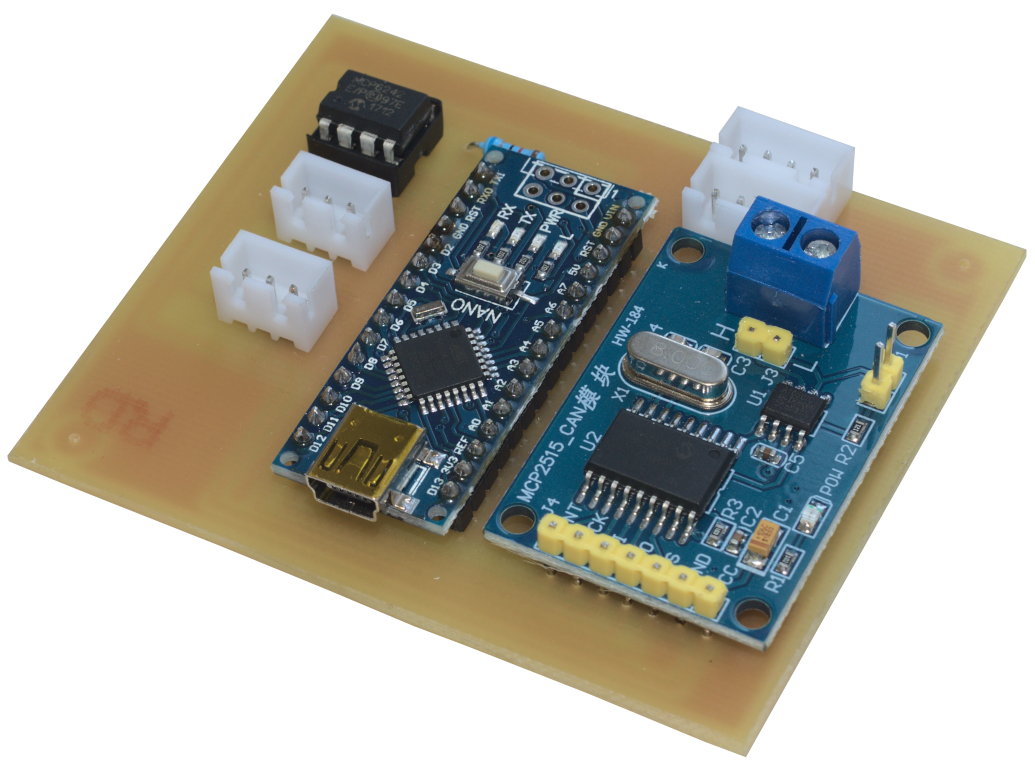
\includegraphics[width=0.9\textwidth]{Fotos/Regler_Platine.png}};
        \begin{scope}[x={(image.south east)},y={(image.north west)}]
            \draw[red,ultra thick,rounded corners,rotate around={-23:(0.68,0.68)}] (0.62,0.67) rectangle (0.8,0.9);
            \draw[blue,ultra thick,rounded corners,rotate around={-20:(0.3,0.68)}] (0.2,0.53) rectangle (0.35,0.7);
            \draw[orange,ultra thick,rounded corners,rotate around={-20:(0.35,0.78)}] (0.26,0.66) rectangle (0.41,0.8);
        \end{scope}
    \end{tikzpicture}
    \captionof{figure}{Platine zur Regleransteuerung}
\end{minipage}
\begin{minipage}{7cm}
    \textcolor{red}{CAN-Bus Anschlüsse}\\
    \textcolor{orange}{Serielle Verbindung zum Regler}\\
    \textcolor{blue}{PWM-Ausgang}\\

\end{minipage}

\subsubsection{Anmerkung:}
Durch die Verwendung der seriellen Schnittstelle des Arduinos muss zur Programmierung der Operationsverstärker entfernt werden.
\newpage

\subsubsection{Schaltplan}
\begin{figure}[h]
    \centering
    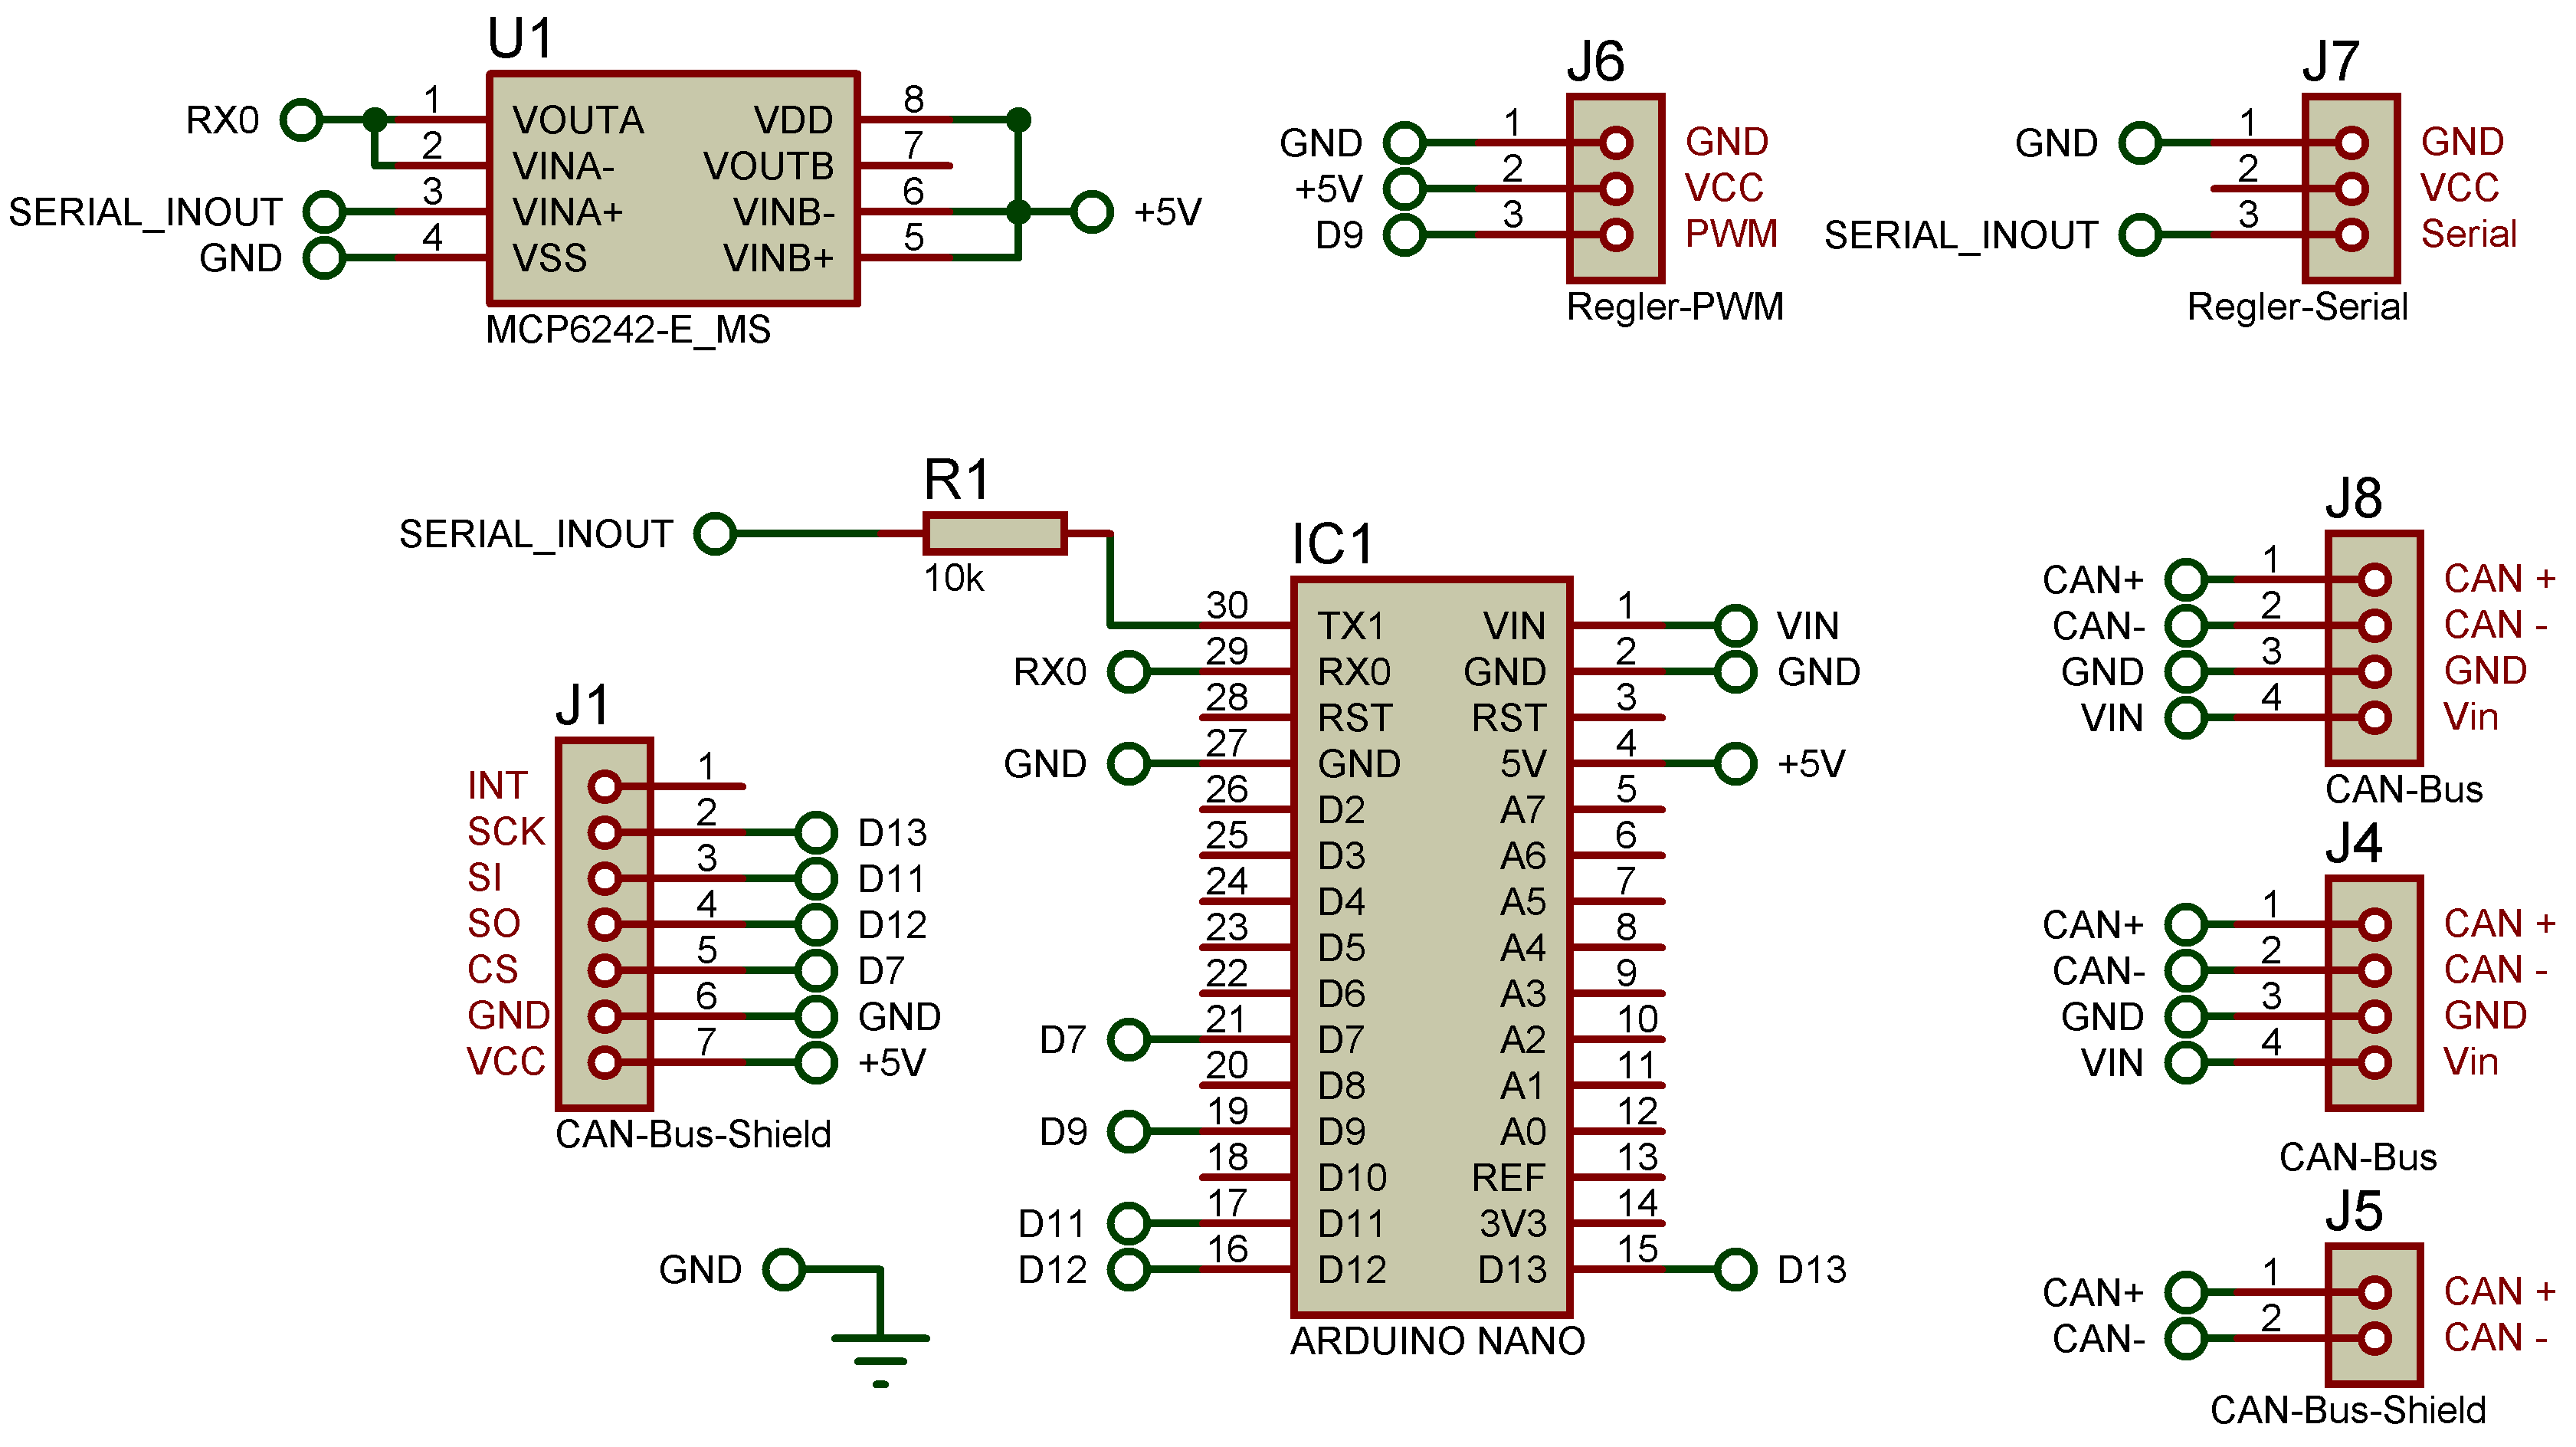
\includegraphics[width=1.0\textwidth]{../Proteus/Exports/Regler-Platine.png}    
    \caption{Schaltplan der Regler-Platine\label{fig:plat:regler}}
\end{figure}

\newpage

\subsubsection{PCB-Layout}
\begin{figure}[h]
    \centering
    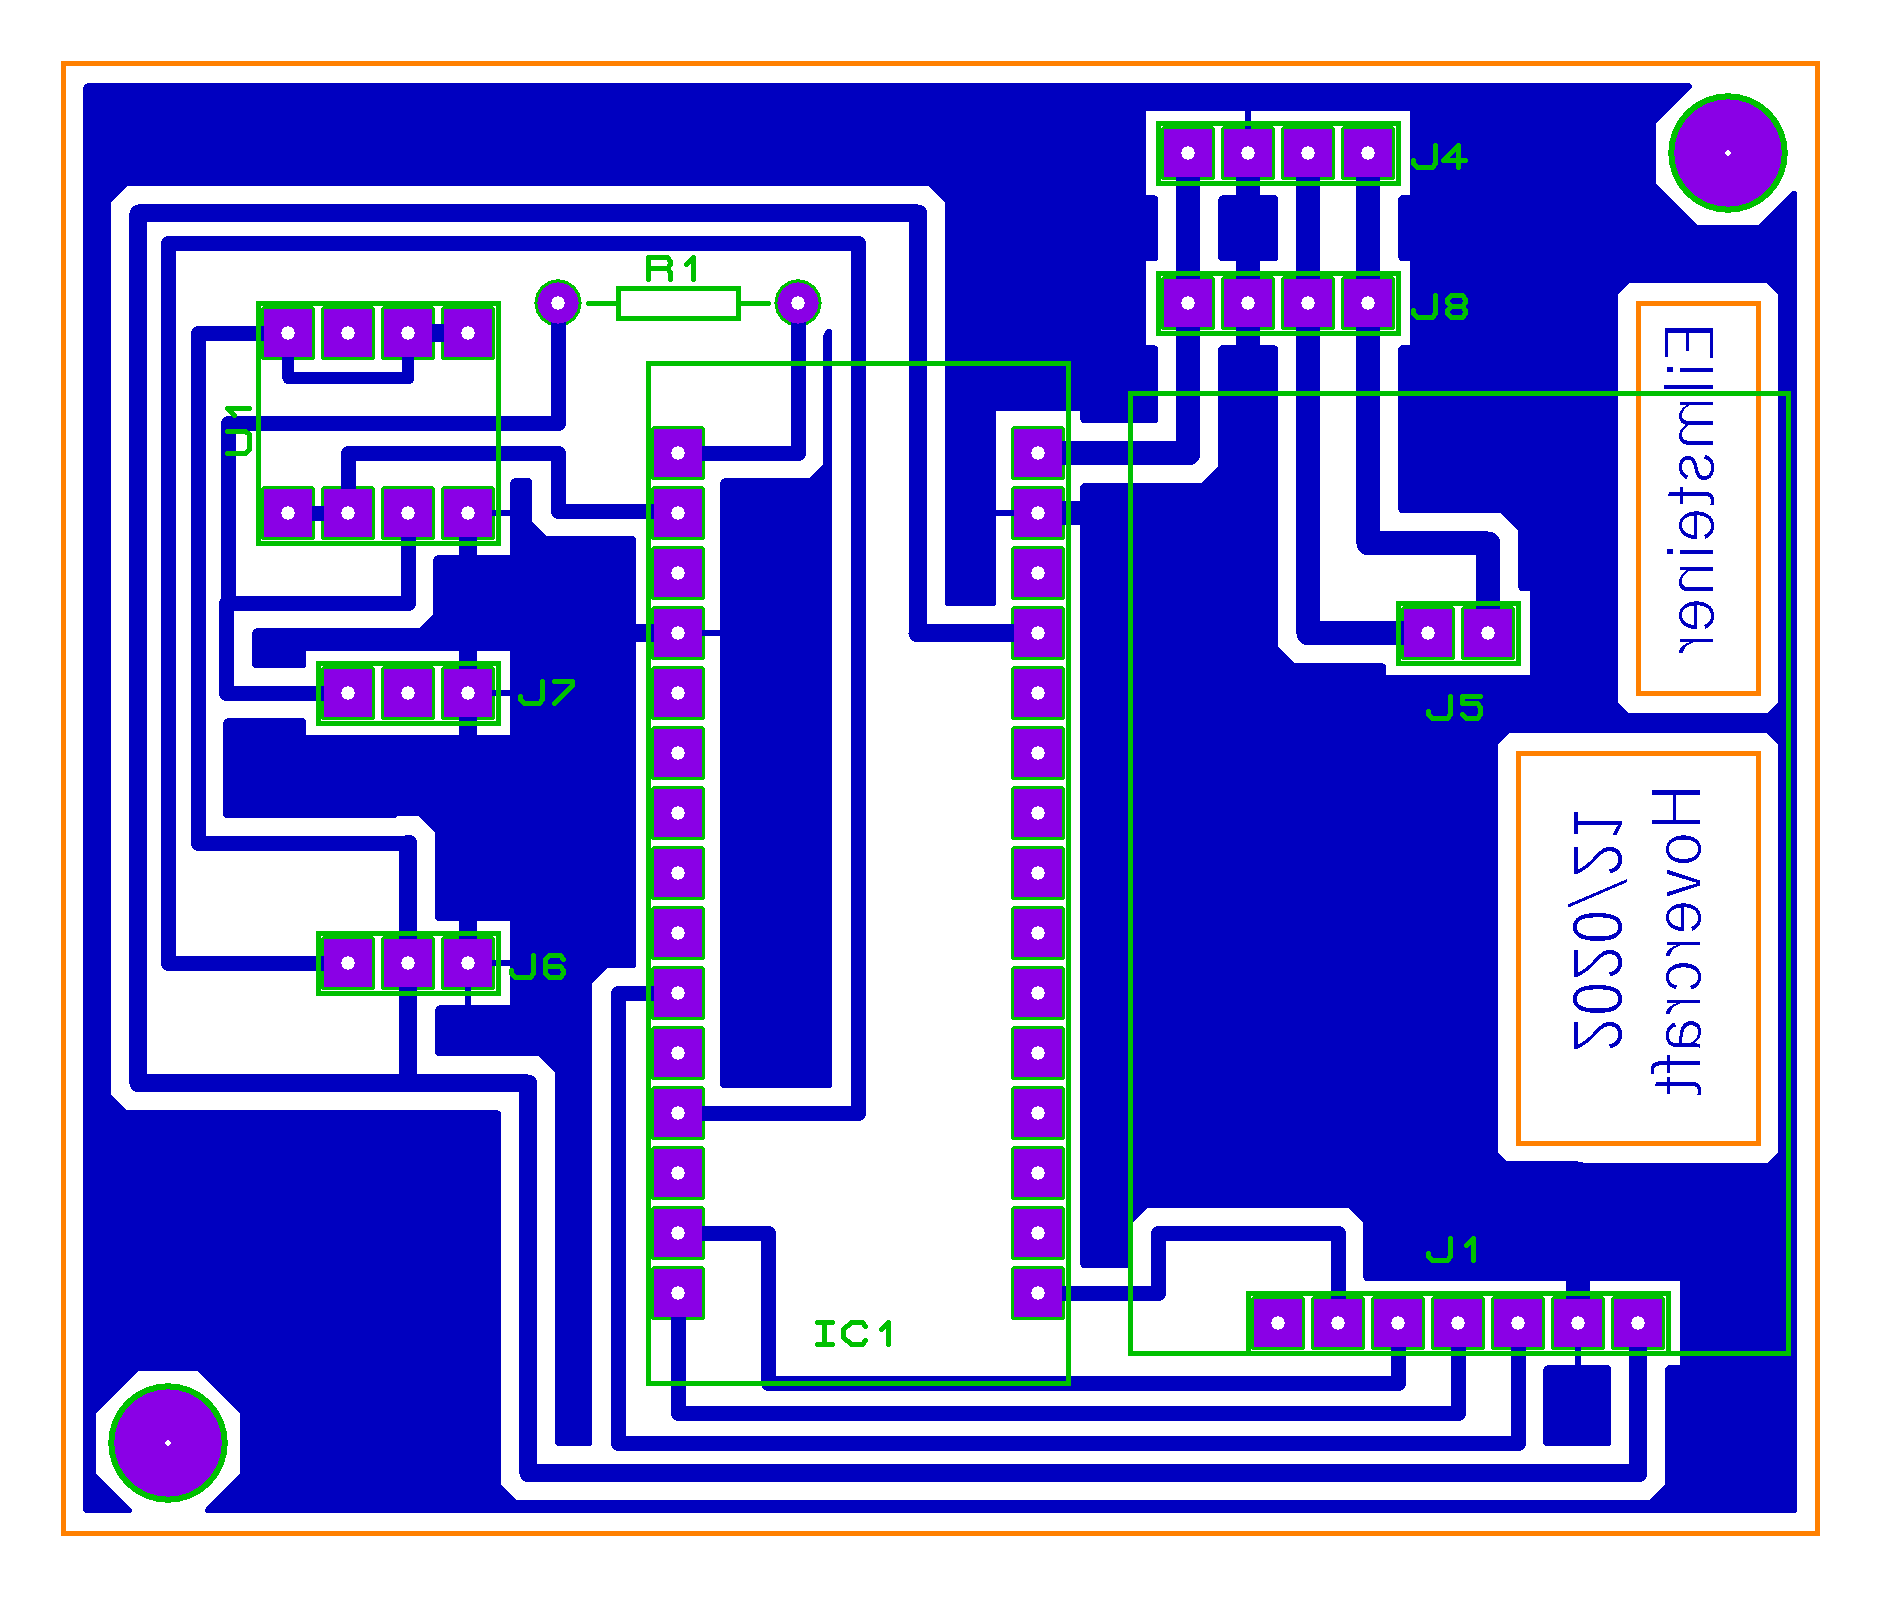
\includegraphics[width=1.0\textwidth]{../Proteus/Exports/Regler_Platine_PCB.png}    
    \caption{PCB-Layout der Regler-Platine}
\end{figure}

\newpage
\subsubsection{Programmcode}
\lstinputlisting{../Programmierung/Regler_Controller/src/main.cpp}
\newpage
\subsection{Lenker\label{sec:Lenkerplatine}}
\subsubsection{Aufgaben \& verwendete Bauteile}
Neben seiner Hauptaufgabe, nämlich dem Einlesen und der Übertragung der beiden Daumengas- sowie Lenkerstellungen, ist dieser Mikrocontroller weiters für die Darstellung der von den verschiedenen Komponenten erhaltenen Telemetriedaten auf dem Bildschirm verantwortlich.
Dazu zählen neben den Informationen über die beiden Motoren vor allem auch die Temperaturen aller verbauten Akkus sowie die per GPS-Modul ermittelte derzeitige Geschwindigkeit.

\begin{minipage}{8.5cm}
    \begin{tikzpicture}
        \node[anchor=south west,inner sep=0] (image) at (0,0) {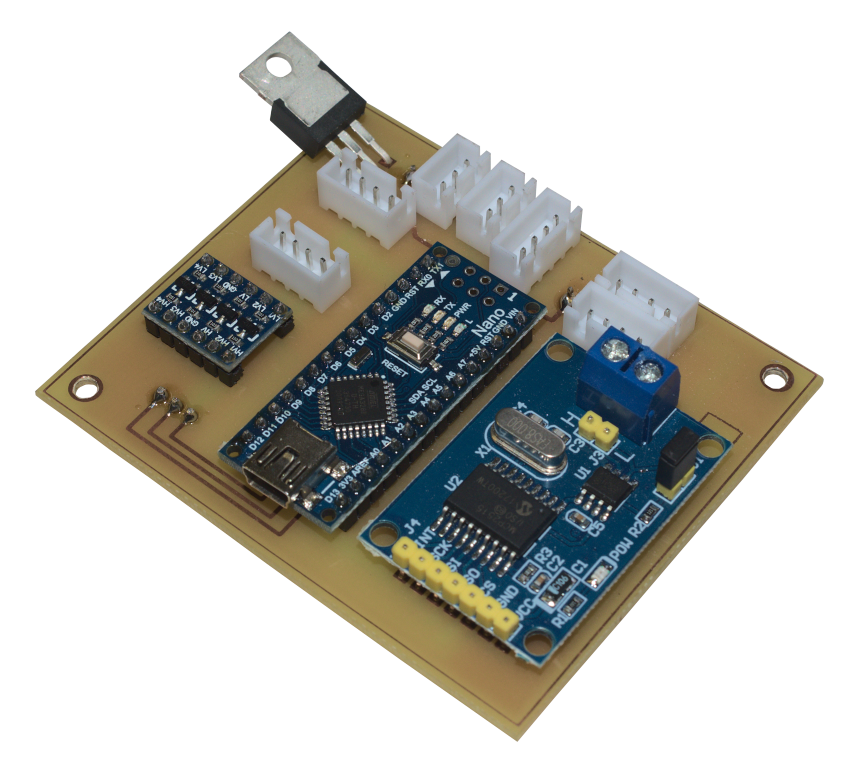
\includegraphics[width=0.9\textwidth]{Fotos/Regler_Lenker.png}};
        \begin{scope}[x={(image.south east)},y={(image.north west)}]
            \draw[red,ultra thick,rounded corners,rotate around={-30:(0.77,0.47)}] (0.6,0.47) rectangle (0.77,0.62);
            \draw[blue,ultra thick,rounded corners,rotate around={-30:(0.4,0.58)}] (0.25,0.58) rectangle (0.4,0.68);
            \draw[orange,ultra thick,rounded corners,rotate around={-30:(0.47,0.67)}] (0.33,0.67) rectangle (0.47,0.76);
            \draw[Green,ultra thick,rounded corners,rotate around={-34:(0.57,0.67)}] (0.45,0.67) rectangle (0.57,0.8);
            \draw[violet,ultra thick,rounded corners,rotate around={-34:(0.62,0.60)}] (0.54,0.60) rectangle (0.62,0.75);
        \end{scope}
    \end{tikzpicture}
    \captionof{figure}{Platine des Lenkers}
\end{minipage}
\begin{minipage}{7cm}
    \textcolor{red}{CAN-Bus Anschlüsse}\\
    \textcolor{blue}{Serielle Verbindung zum GPS-Modul}\\
    \textcolor{orange}{Serielle Verbindung zum Bildschirm}\\
    \textcolor{Green}{Daumengas Anschlüsse}\\
    \textcolor{violet}{Anschluss Lenkerpotenziometer}\\

\end{minipage}

\vspace{0.5cm}
\begin{minipage}{7.5cm}
    \centering
    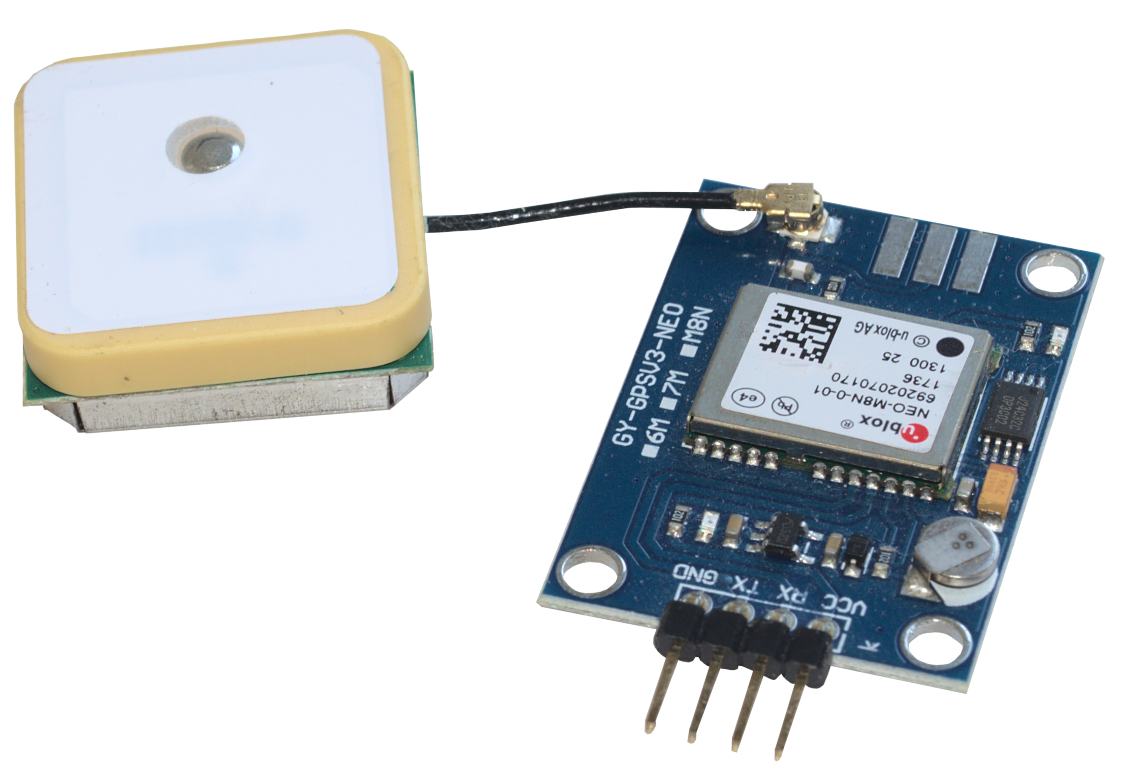
\includegraphics[width=0.99\textwidth]{Fotos/GPS_Modul_2.png}
    \captionof{figure}{NEO-8M GPS-Modul}
\end{minipage}
\hspace{0.1cm}
\begin{minipage}{7.5cm}
    \centering
    \includegraphics[width=0.99\textwidth]{Fotos/Daumengas_2.png}
    \captionof{figure}{Daumengas}
\end{minipage}

\newpage

\subsubsection{Schaltplan}
\begin{figure}[h]
    \centering
    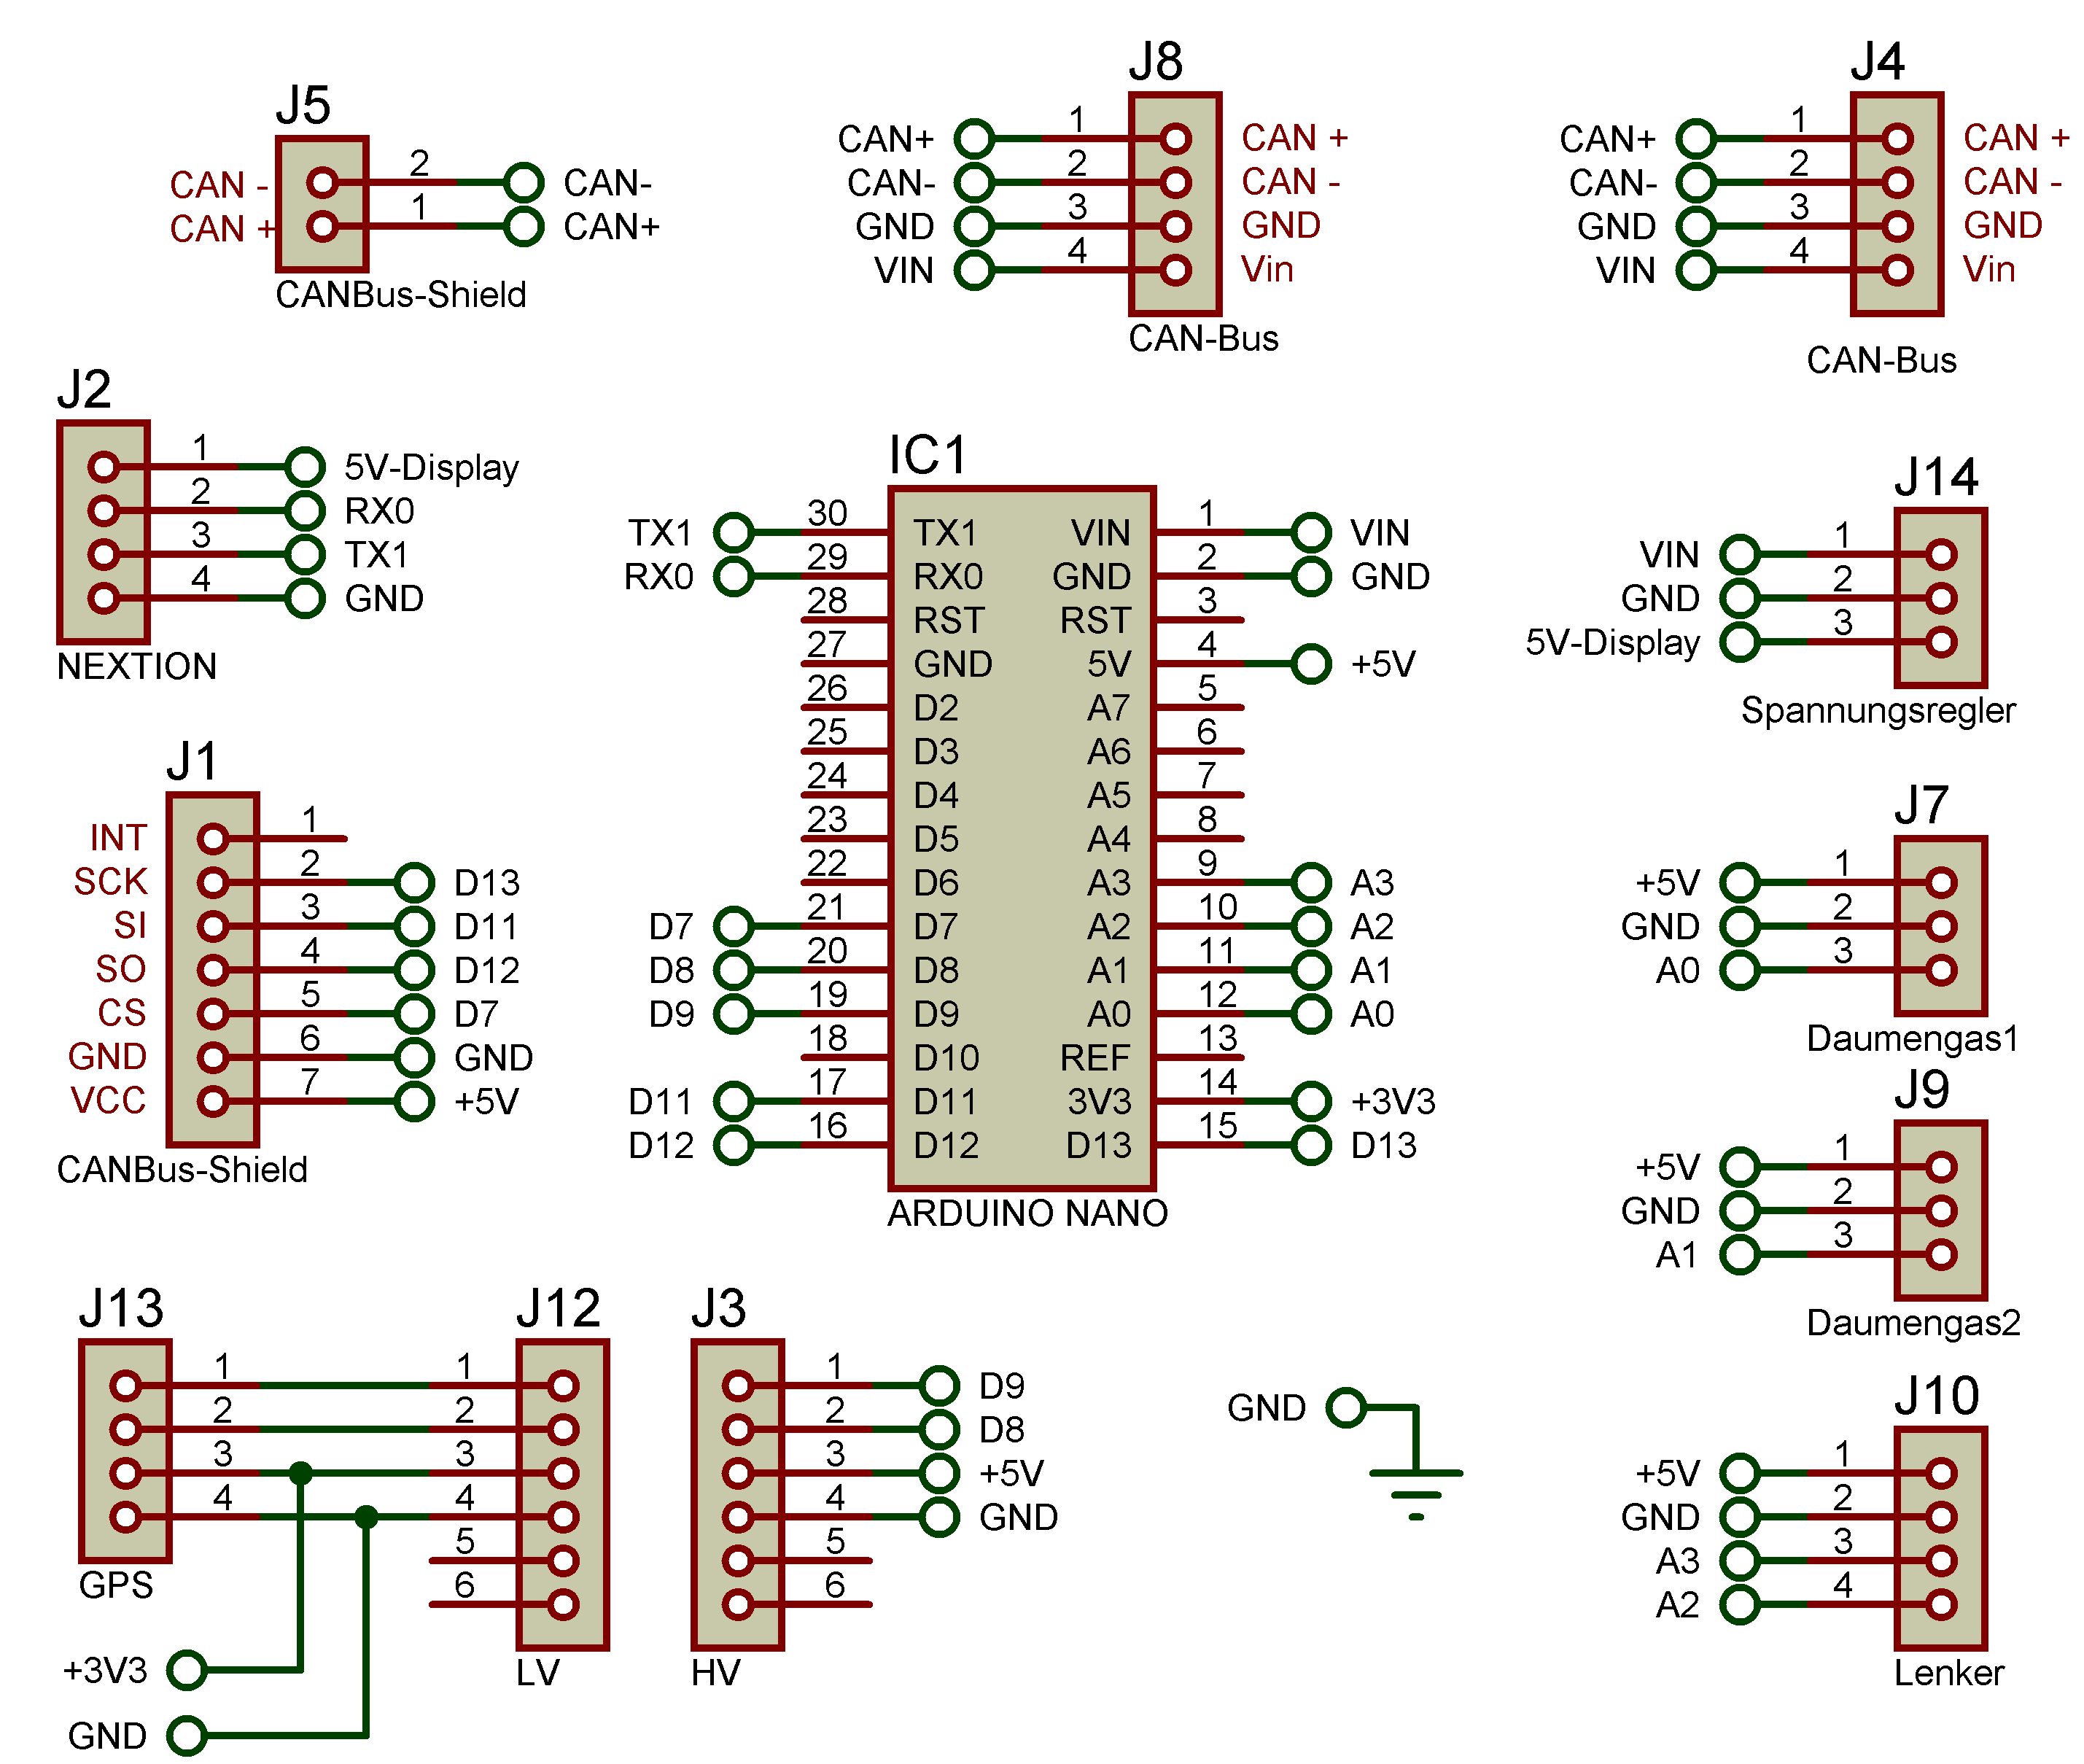
\includegraphics[width=1.0\textwidth]{../Proteus/Exports/Lenker-Platine.png}    
    \caption{Schaltplan der Lenker-Platine\label{fig:plat:lenker}}
\end{figure}

\newpage

\subsubsection{PCB-Layout}
\begin{figure}[h]
    \centering
    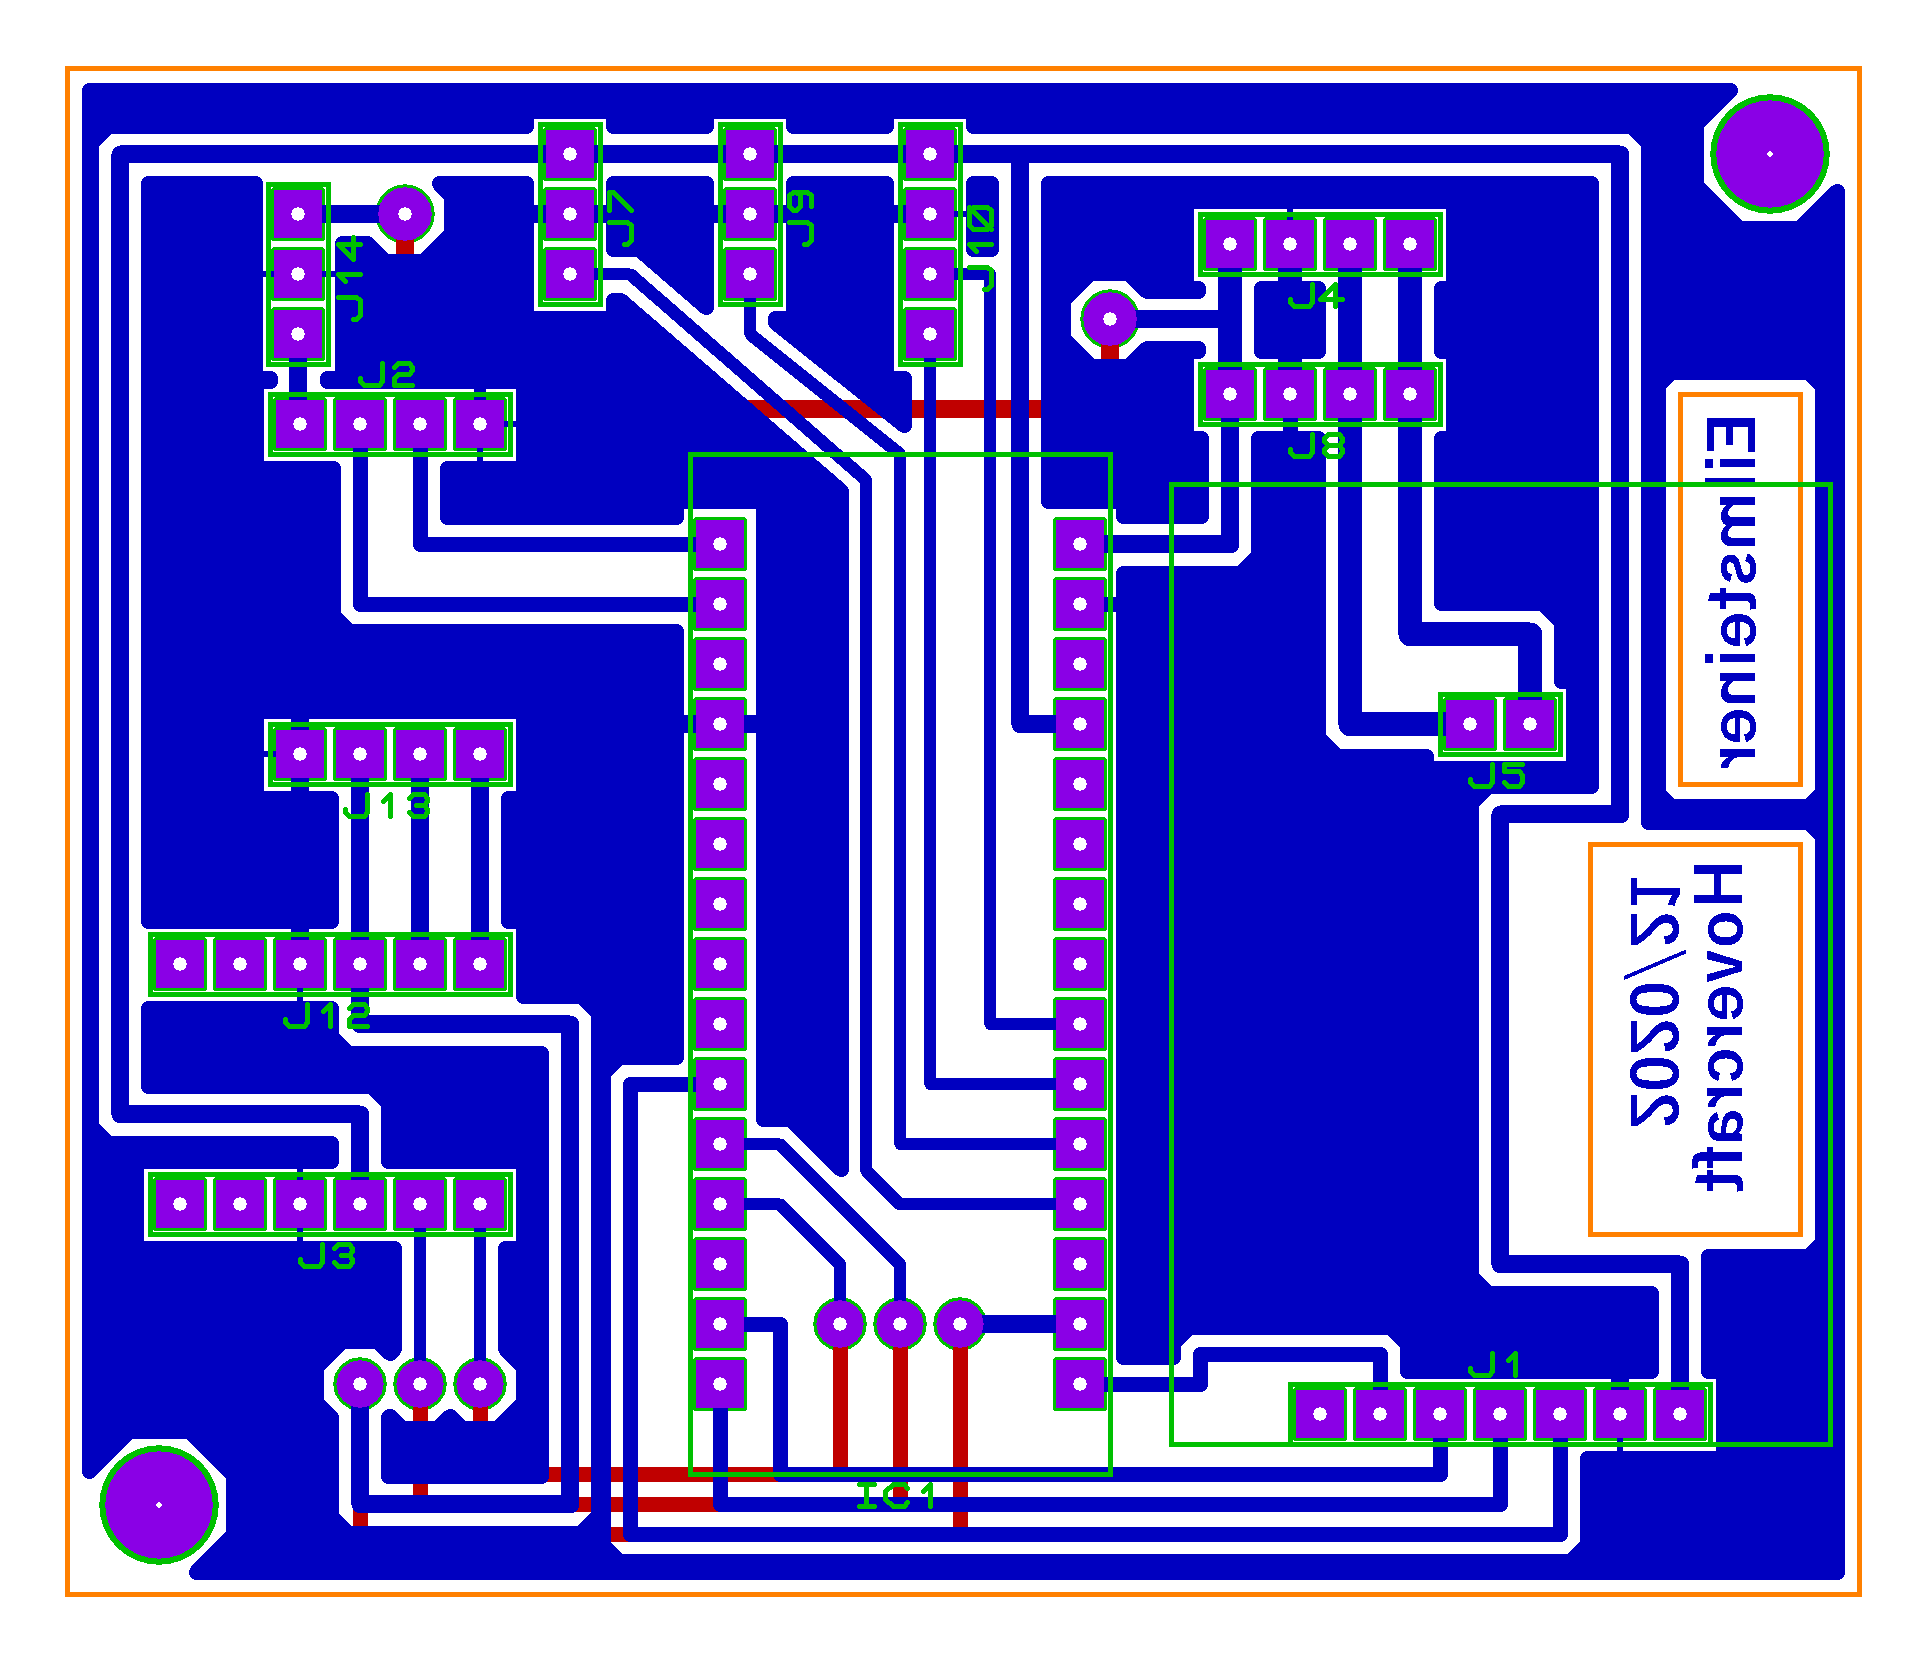
\includegraphics[width=1.0\textwidth]{../Proteus/Exports/Lenker_Platine_PCB.png}    
    \caption{PCB-Layout der Lenker-Platine}
\end{figure}

\newpage
\subsubsection{Programmcode}
\lstinputlisting{../Programmierung/Lenker_Controller/src/main.cpp}

\newpage

\subsection{Fahnenansteuerung \&\ Akkutemperaturen\label{sec:Servoplatine}}
\subsubsection{Fahnenansteuerung}
Die Ansteuerung der Servos erfolgt ebenfalls mit einem per CAN-Bus angeschlossenen Arduino. Um die für die Steuerung der drei Servos benötigten PWM-Signale unabhängig von den durch den Arduino bereitgestellten Timer und den damit verbundenen GPIOs zu erzeugen 
(Anbindung des CAN-Bus Moduls über SPI benötigt beispielsweise diese Pins und Timer), wurde dafür auf ein externes Board zurückgegriffen.

\begin{minipage}{8.5cm}
    \begin{tikzpicture}
        \node[anchor=south west,inner sep=0] (image) at (0,0) {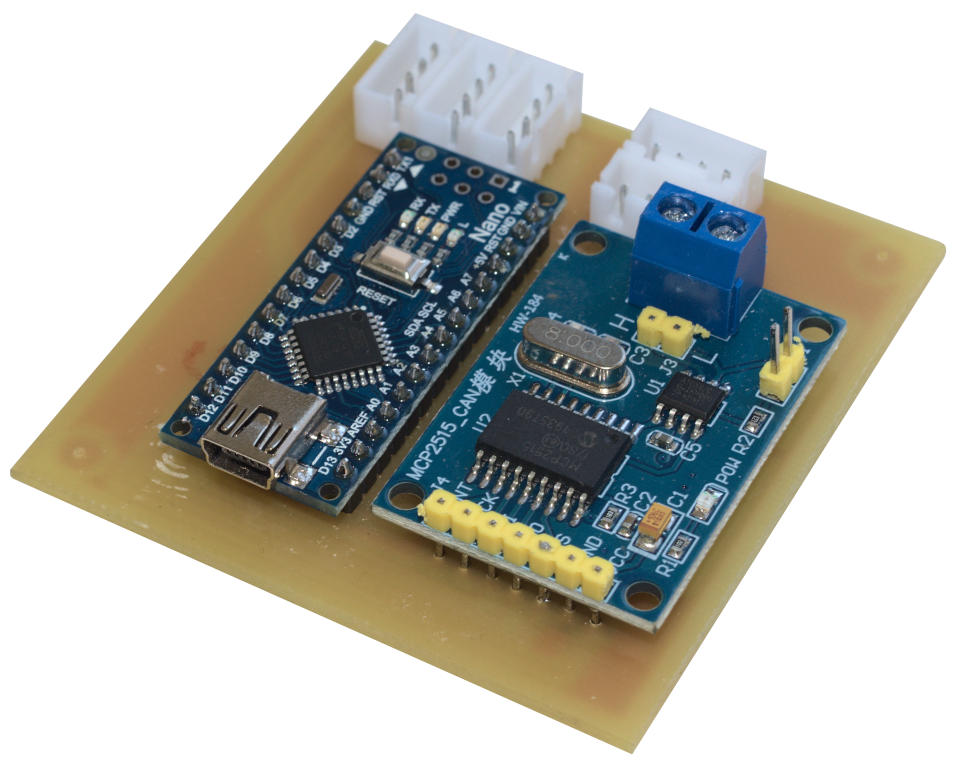
\includegraphics[width=0.9\textwidth]{Fotos/Regler_Servos.png}};
        \begin{scope}[x={(image.south east)},y={(image.north west)}]
            \draw[red,ultra thick,rounded corners,rotate around={-23:(0.64,0.68)}] (0.58,0.67) rectangle (0.78,0.9);
            \draw[blue,ultra thick,rounded corners,rotate around={-20:(0.5,0.9)}] (0.37,0.76) rectangle (0.63,0.99);
        \end{scope}
    \end{tikzpicture}
    \captionof{figure}{Platine zur Regleransteuerung}
\end{minipage}
\begin{minipage}{7cm}
    \textcolor{red}{CAN-Bus Anschlüsse}\\
    \textcolor{blue}{I2C Anschlüsse}\\
    
\end{minipage}\\

Konkret handelt es sich um das \textbf{16-Channel 12-bit PWM/Servo Driver Module} von Adafruit, welcher mittels I2C mit dem Mikrocontroller kommuniziert.\\
\begin{figure}[h]
    \centering
    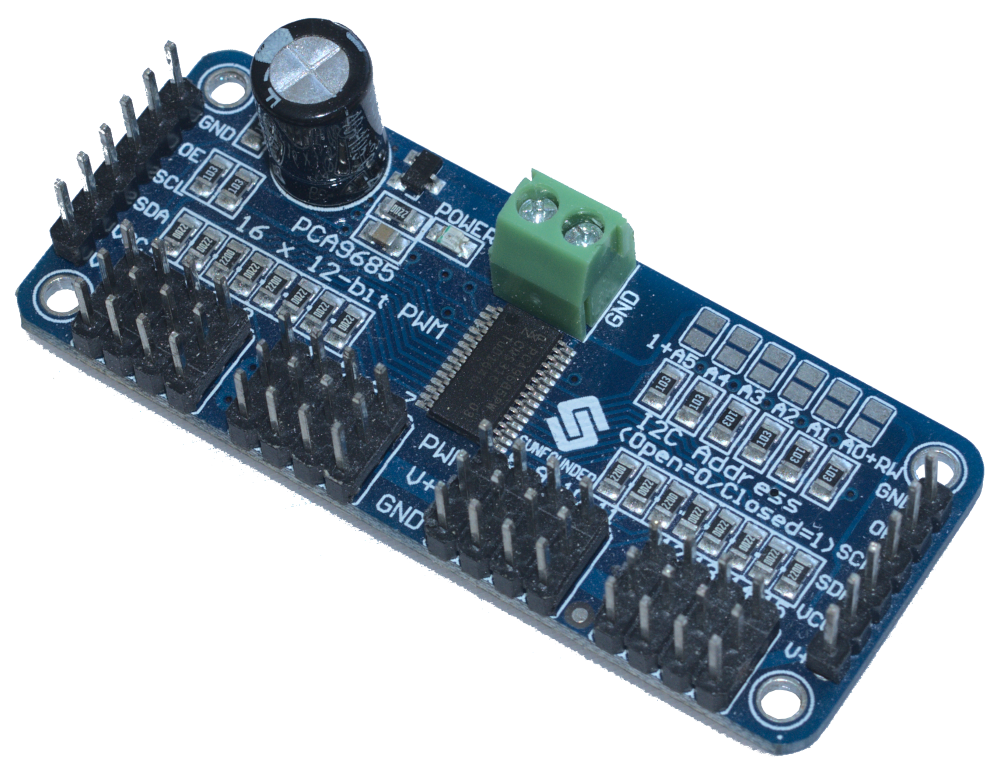
\includegraphics[width=0.5\textwidth]{Fotos/Servo_Controller.png}
    \caption{Adafruit 16-Channel Servo Driver}
\end{figure}

\newpage
\subsubsection{Schaltplan}
\begin{figure}[h]
    \centering
    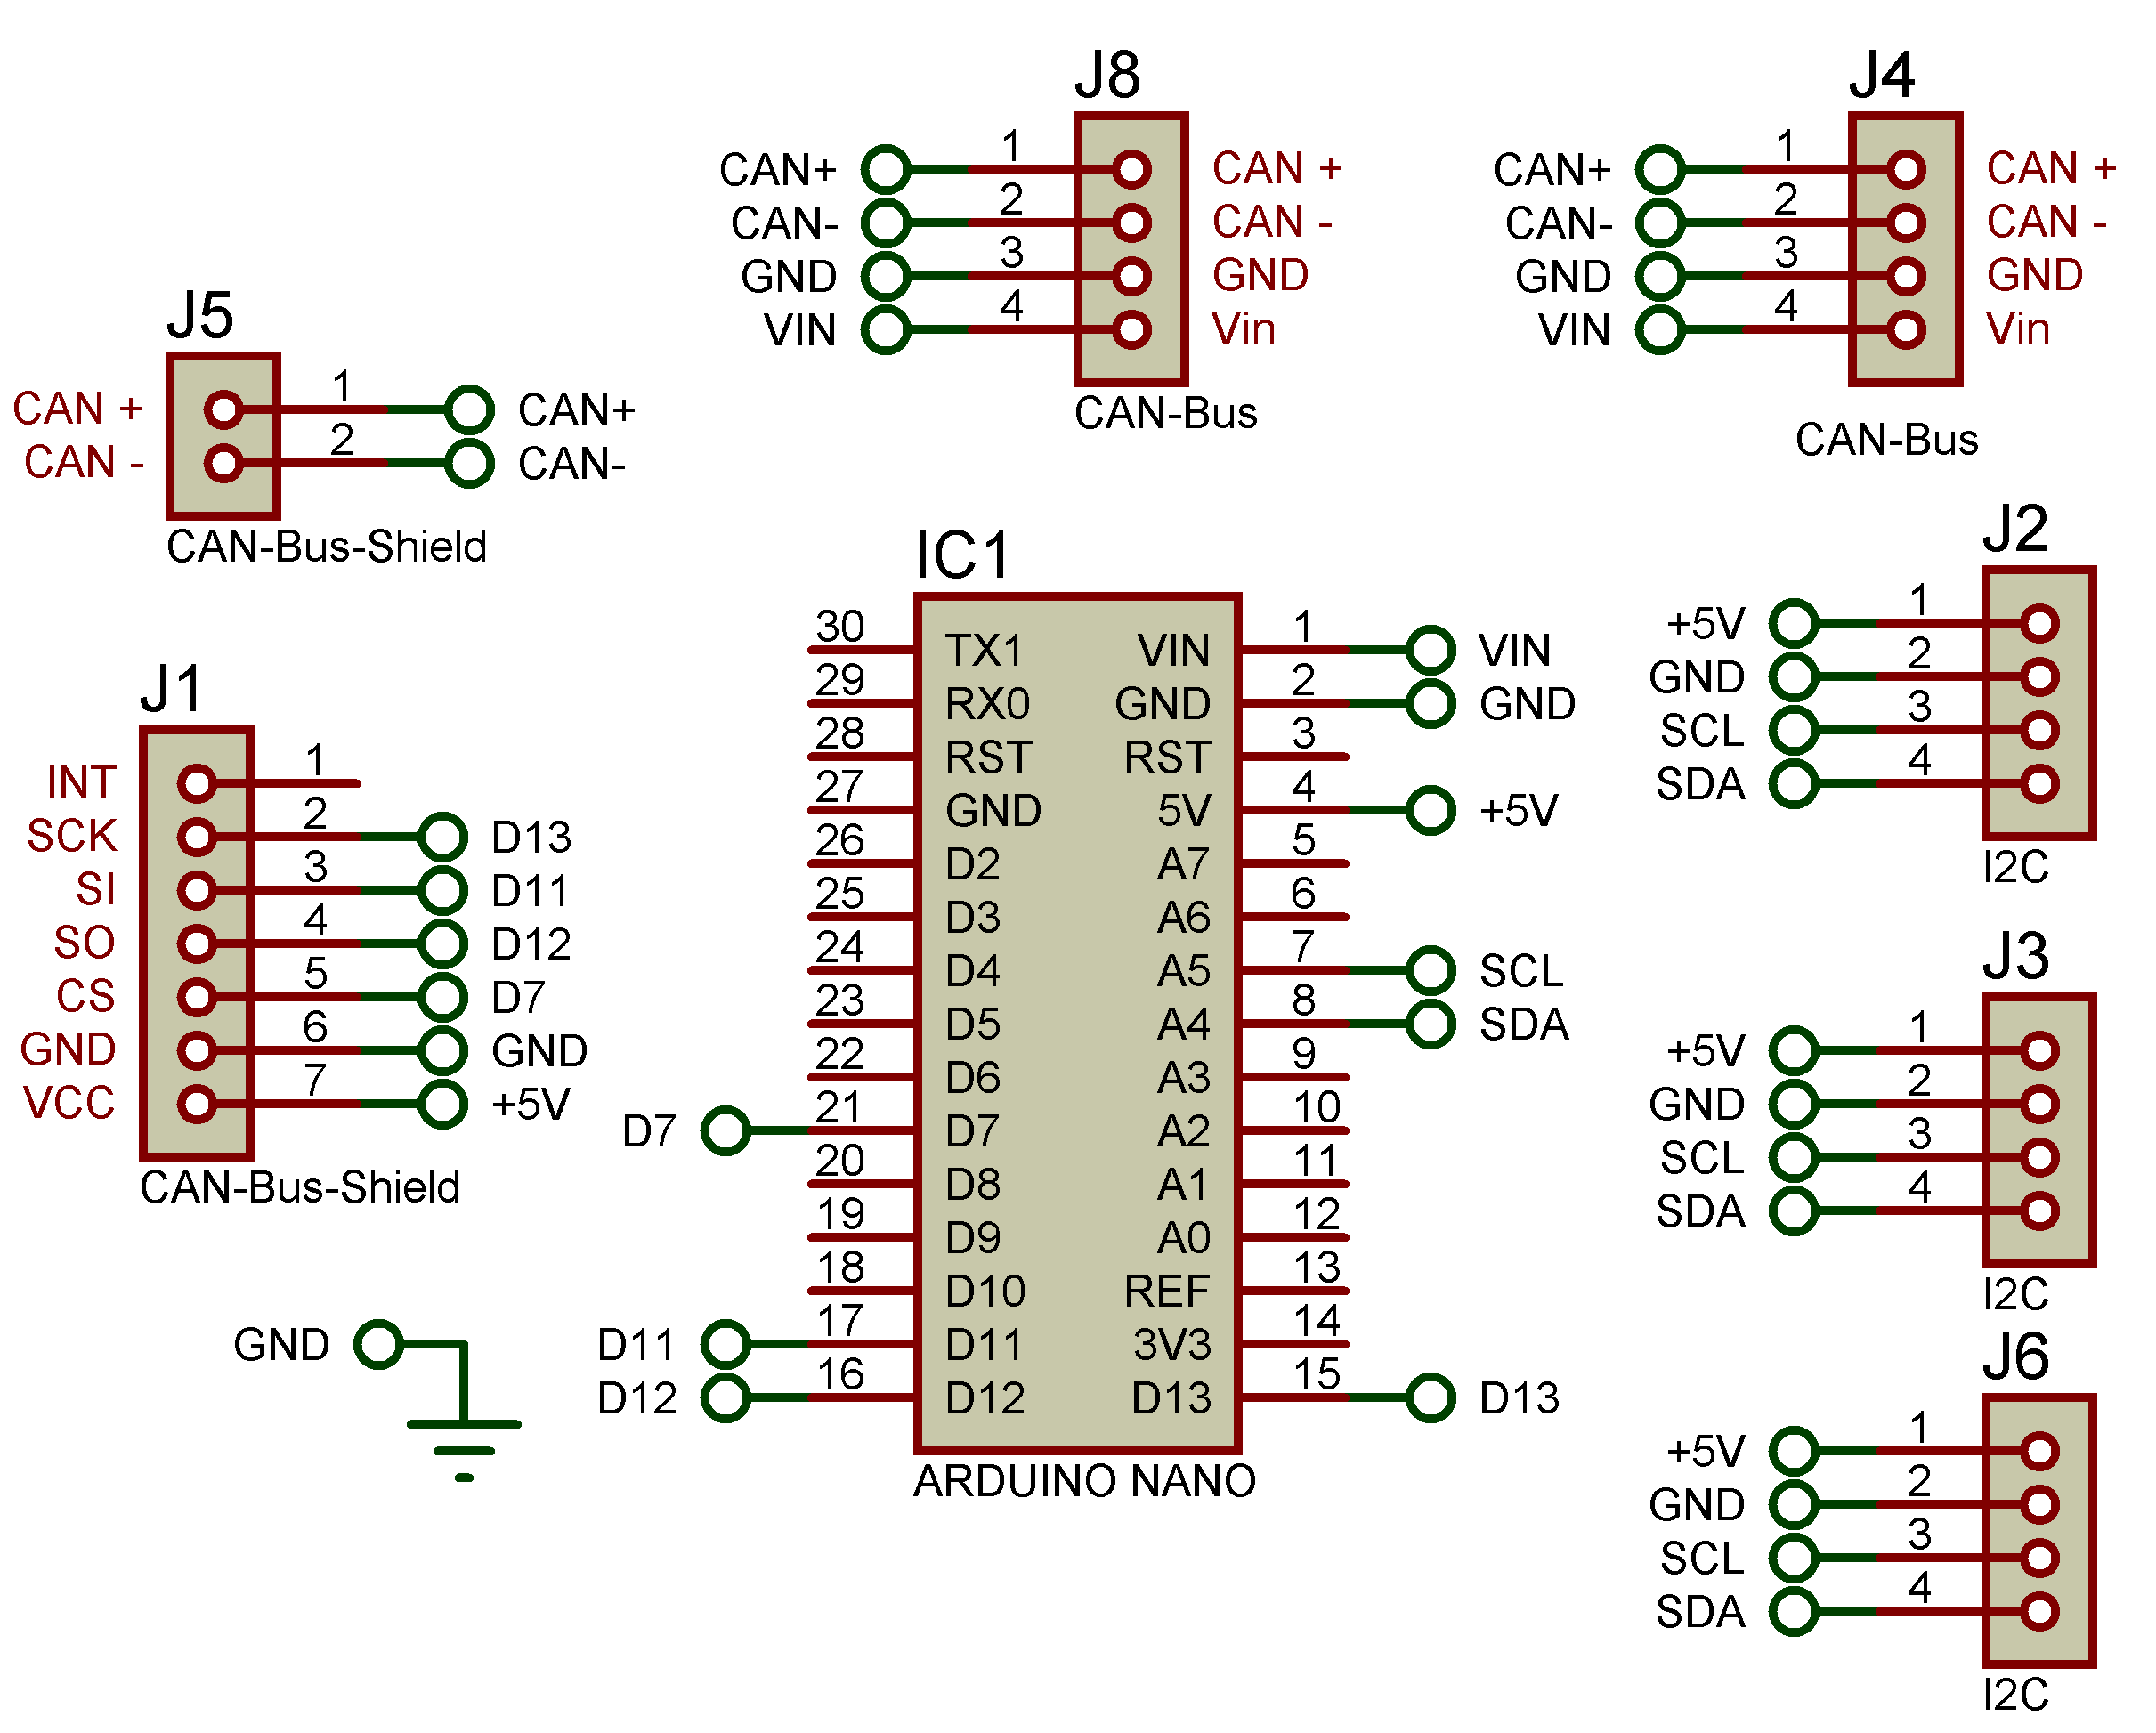
\includegraphics[width=1.0\textwidth]{../Proteus/Exports/Servos-Platine.png}    
    \caption{Schaltplan der Servoansteuerung-Platine\label{fig:plat:servo}}
\end{figure}

\newpage
\subsubsection{PCB-Layout}
\begin{figure}[h]
    \centering
    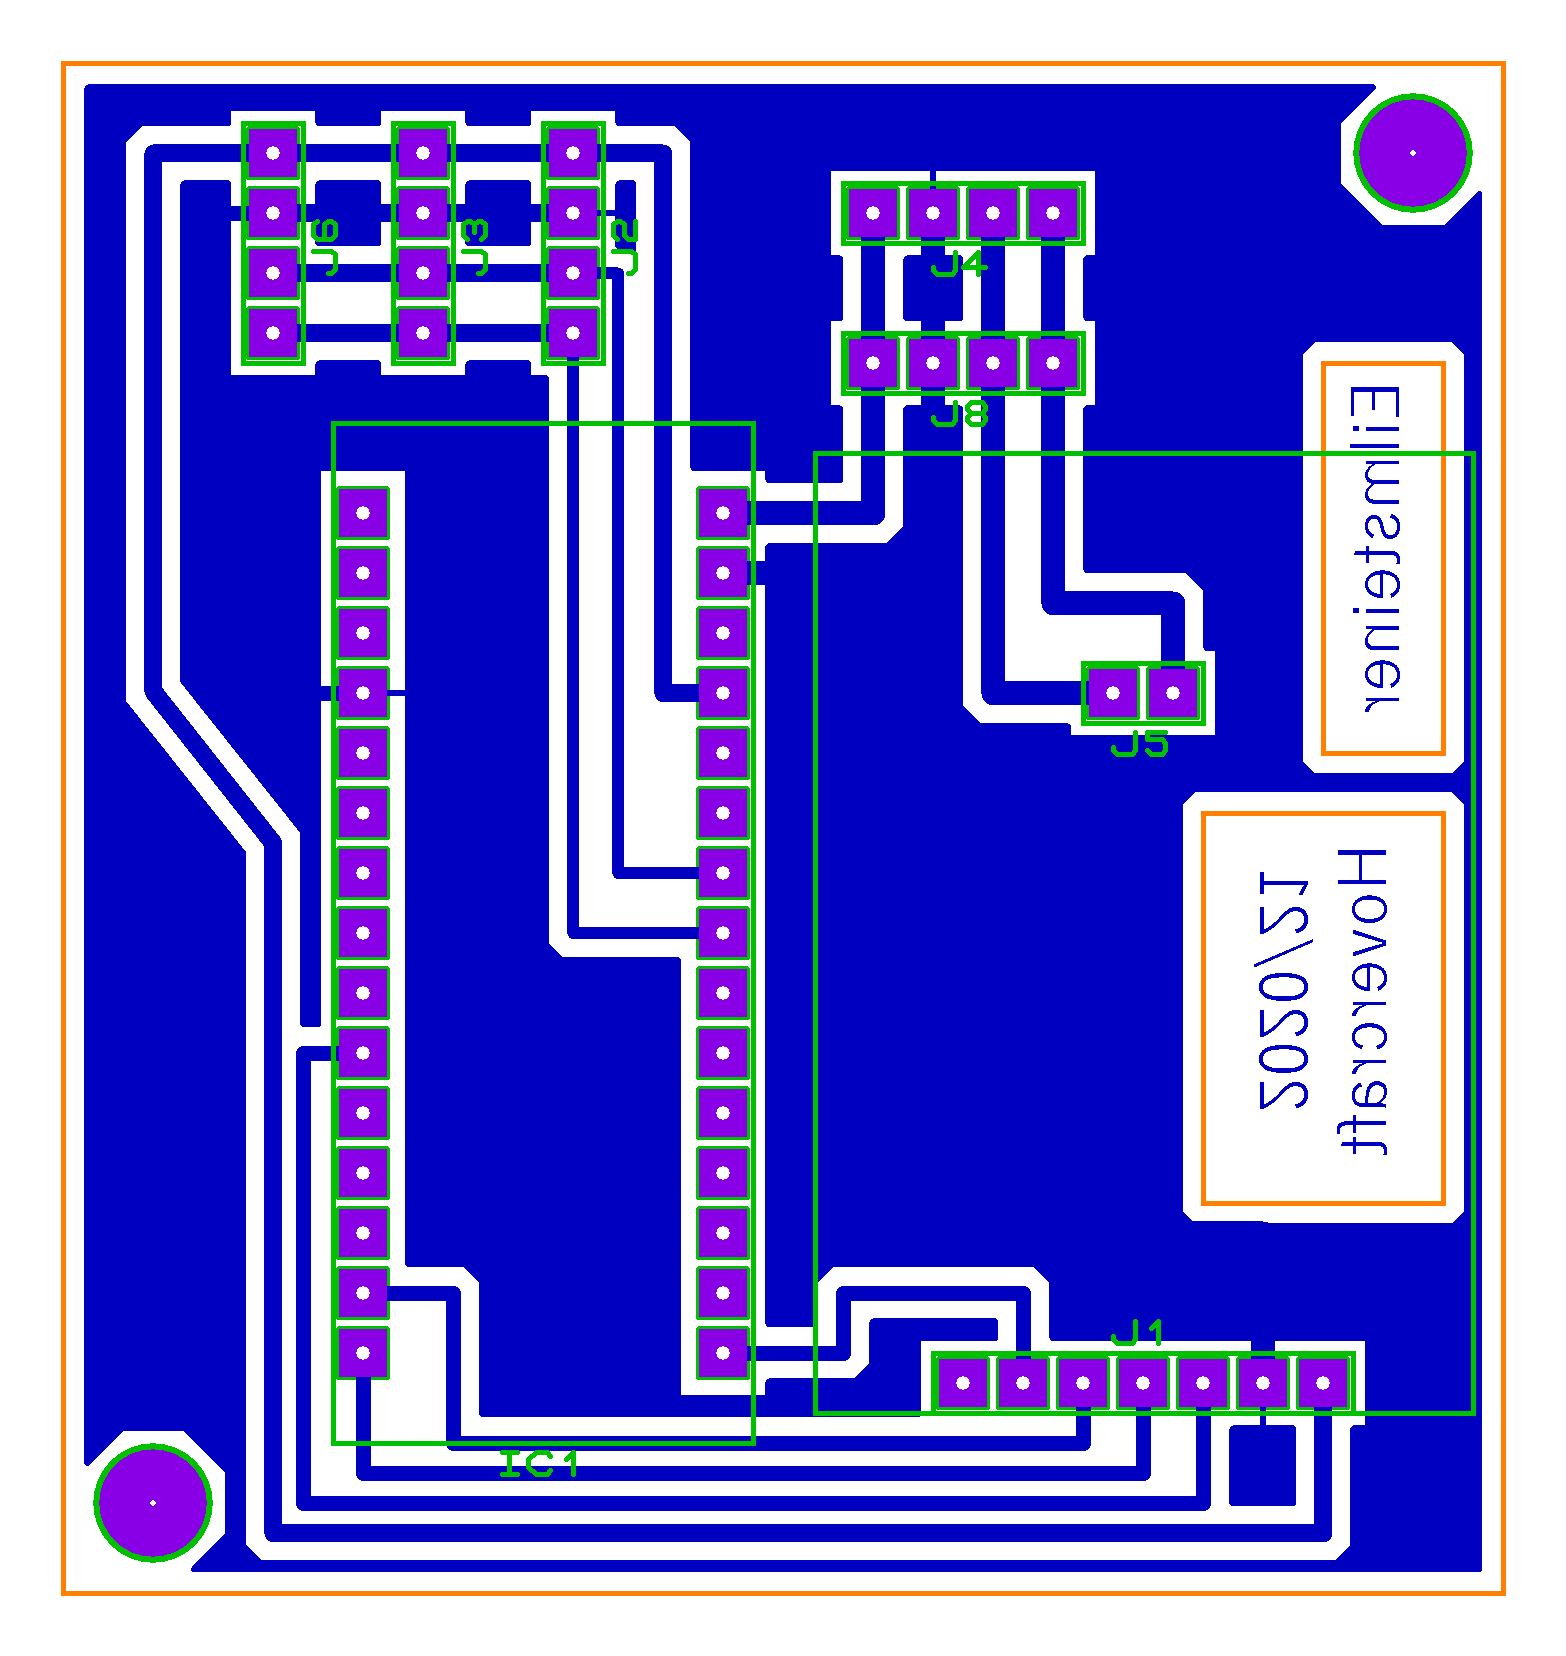
\includegraphics[width=0.9\textwidth]{../Proteus/Exports/Servos-Platine-PCB.png}    
    \caption{PCB-Layout der Servoansteuerung-Platine}
\end{figure}

\newpage
\subsubsection{Programmcode}
\lstinputlisting{../Programmierung/Servo_ADC_Controller/src/main.cpp}
\newpage

\subsubsection{Akkutemperaturen}
Die zweite Aufgabe dieses Controllers ist es, die Temperaturen aller acht im Boot verbauten Akkus zu überwachen, und diese zur Darstellung an den Controller des Lenkers zu übermitteln.
Dies geschieht mithilfe zweier (je einer pro Seite), ebenfalls über I2C verbundenen, \textbf{ADS1115} Analog-Digital-Wandler, welche wiederum von Adafruit stammen.\\
Zur Temperaturmessung selbst kommt je ein \textbf{LM35} Temperatursensor pro Akku zum Einsatz.\\

\begin{minipage}{8cm}
    \centering
    \includegraphics[width=0.85\textwidth]{Fotos/ADS1115_2.png}
    \captionof{figure}{ADS1115 Modul}    
\end{minipage}
\begin{minipage}{8cm}
    \centering
    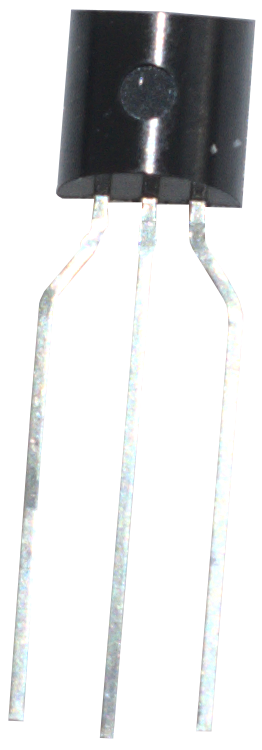
\includegraphics[width=0.17\textwidth]{Fotos/LM35.png}
    \captionof{figure}{LM35}
\end{minipage}\\
\vspace{0.5cm}

\subsection{ADC-Platinen}
Um den Anschluss der Temperatursensoren an diesem ADC zu vereinfachen, wurde folgende Platine entworfen:\\ 
\begin{minipage}{9cm}
    \begin{tikzpicture}
        \node[anchor=south west,inner sep=0] (image) at (0,0) {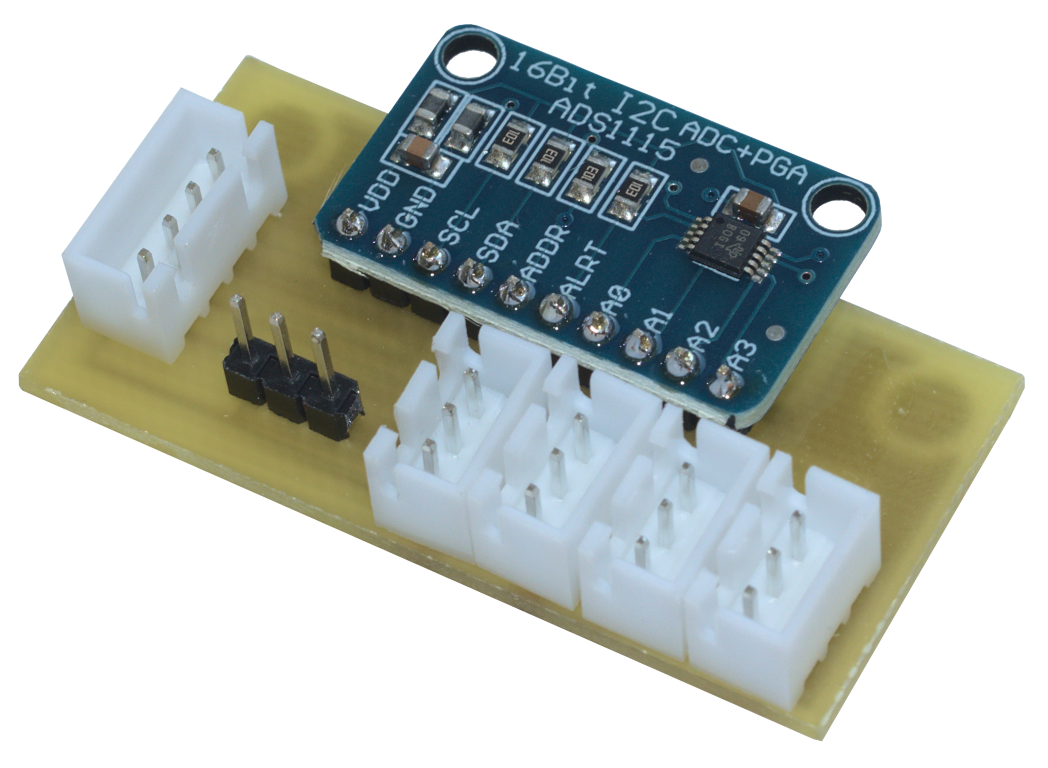
\includegraphics[width=0.9\textwidth]{Fotos/ADC_Platine.png}};
        \begin{scope}[x={(image.south east)},y={(image.north west)}]
            \draw[red,ultra thick,rounded corners,rotate around={-23:(0.78,0.0)}] (0.25,0.0) rectangle (0.78,0.4);
            \draw[blue,ultra thick,rounded corners,,rotate around={-30:(0.00,0.59)}] (0.00,0.59) rectangle (0.20,0.99);
            \draw[Green,ultra thick,rounded corners,,rotate around={-27:(0.3,0.4)}] (0.15,0.4) rectangle (0.34,0.57);
        \end{scope}
    \end{tikzpicture}
    \captionof{figure}{Platine Temperatursensoren}
\end{minipage}
\begin{minipage}{7cm}
    \textcolor{red}{Analogeingänge}\\
    \textcolor{blue}{I2C Anschluss}\\
    \textcolor{Green}{I2C Adressen-Jumper}\\
\end{minipage}\\

\newpage
\subsubsection{Schaltplan}
\begin{figure}[h]
    \centering
    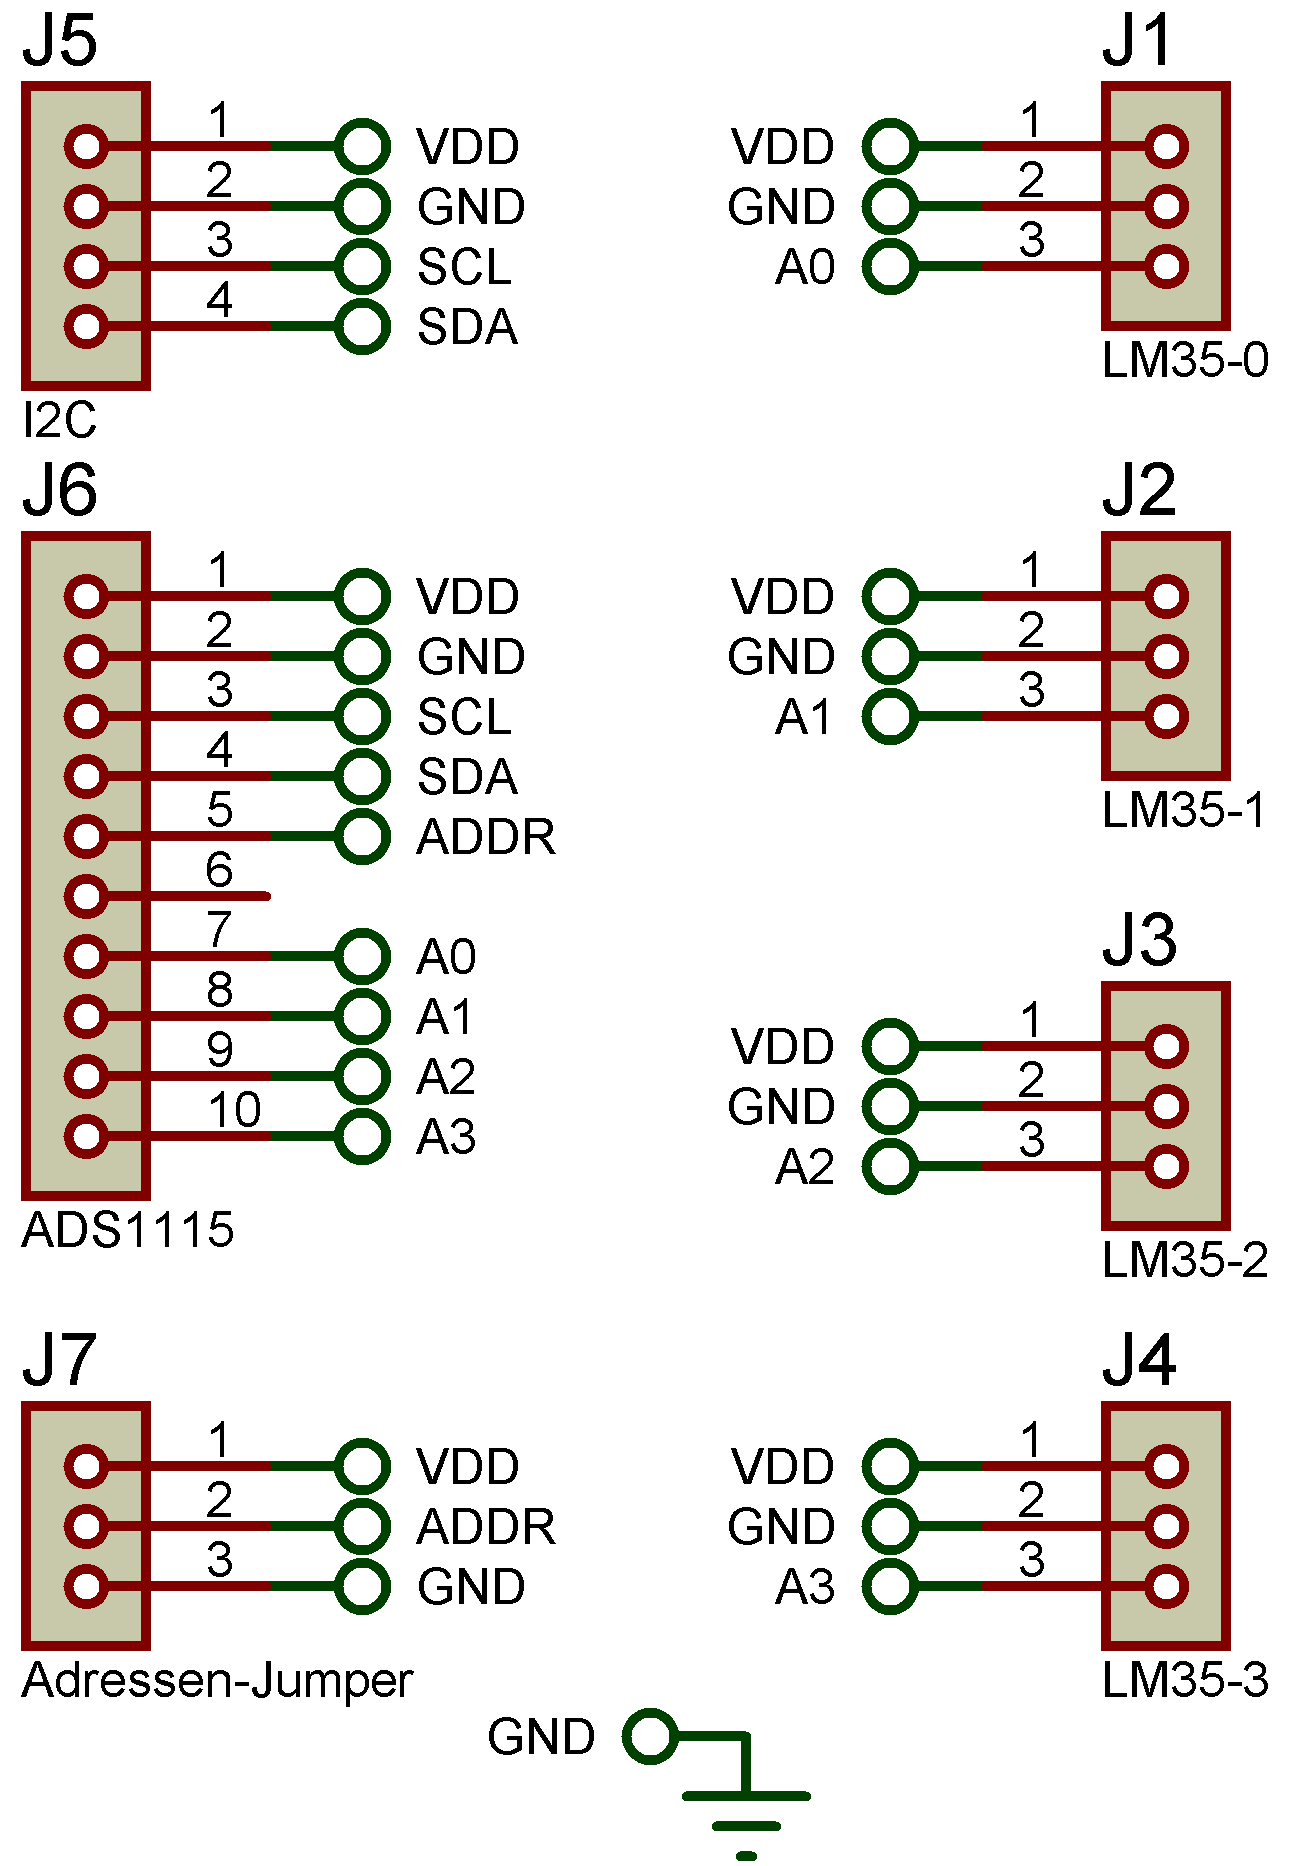
\includegraphics[width=0.6\textwidth]{../Proteus/Exports/Temperatursensoren-Platine.png}    
    \caption{Schaltplan der Temperatursensoren-Platine\label{fig:plat:temp}}
\end{figure}

\newpage

\subsubsection{PCB-Layout}
\begin{figure}[h]
    \centering
    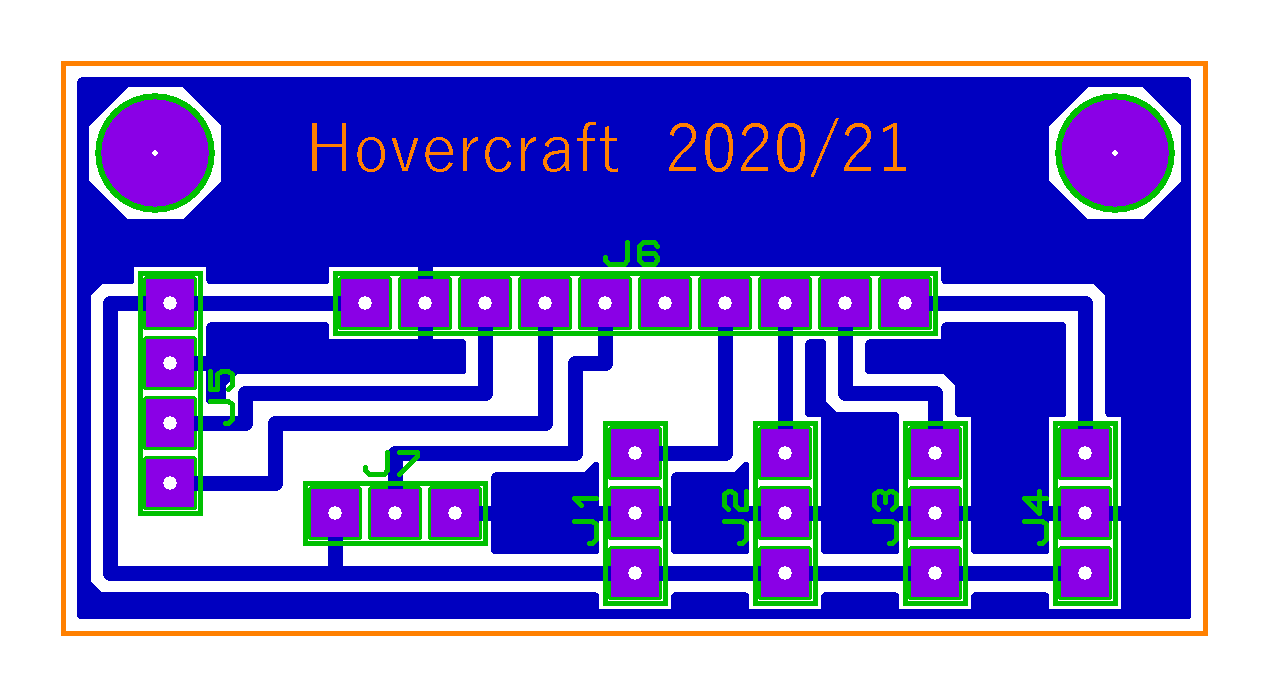
\includegraphics[width=0.8\textwidth]{../Proteus/Exports/Temperatursensoren-Platine-PCB.png}    
    \caption{PCB-Layout der Temperatursensoren-Platine}
\end{figure}

\newpage
\subsection{Precharge \& Relaisansteuerung\label{sec:precharge}}
Da sowohl die Motorregler als auch die Buck-Converter einen, bedingt durch die darin verbauten sehr großen Kondensatoren, sehr großen Einschaltstrom haben, 
müssen diese über einen Leistungswiderstand vorgeladen werden, bevor sie permanent mit Spannung versorgt werden können.\\
\begin{figure}[h]
    \centering
    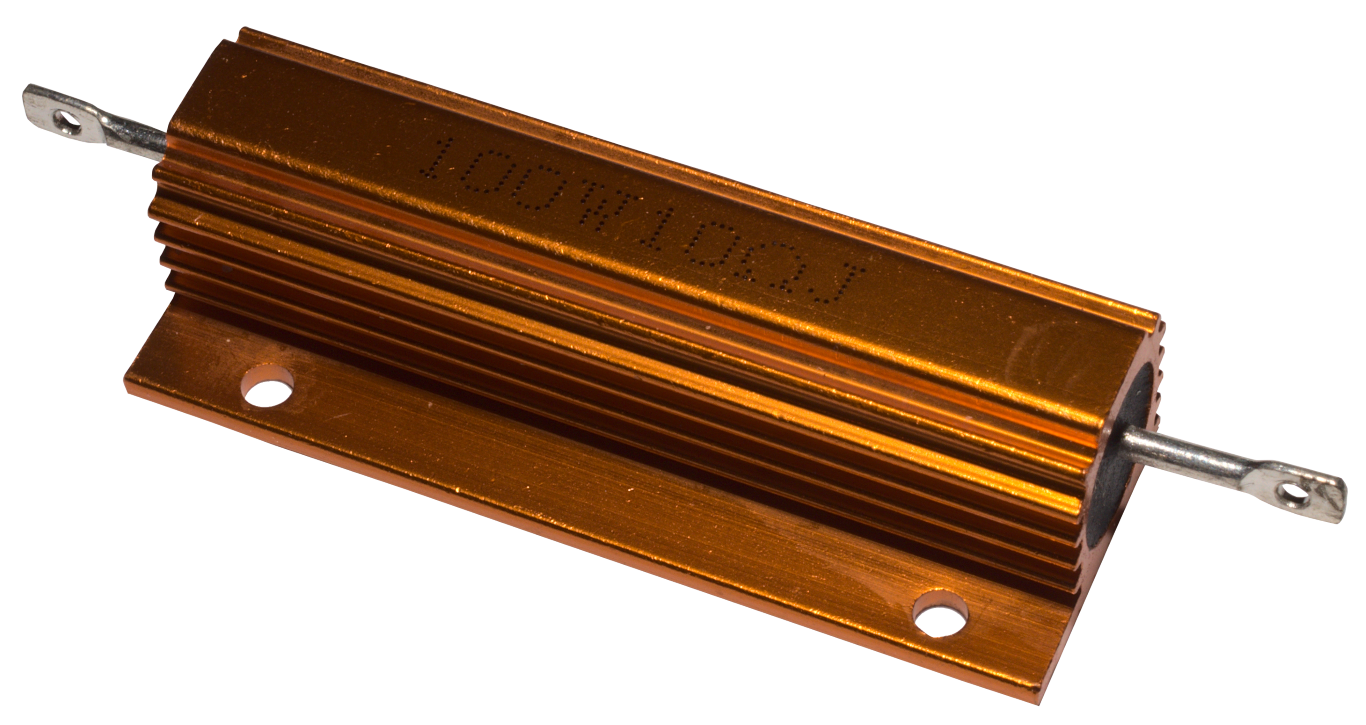
\includegraphics[width=0.55\textwidth]{Fotos/Leistungswiderstand.png}
    \caption{Zur Vorladung verwendeter Leistungswiderstand}
\end{figure}

Um diese Umschaltung so einfach wie möglich zu gestalten, wurde dies mithilfe einer im Folgenden genauer erläuterten Platine realisiert. 

\begin{minipage}{9cm}
    \begin{tikzpicture}
        \node[anchor=south west,inner sep=0] (image) at (0,0) {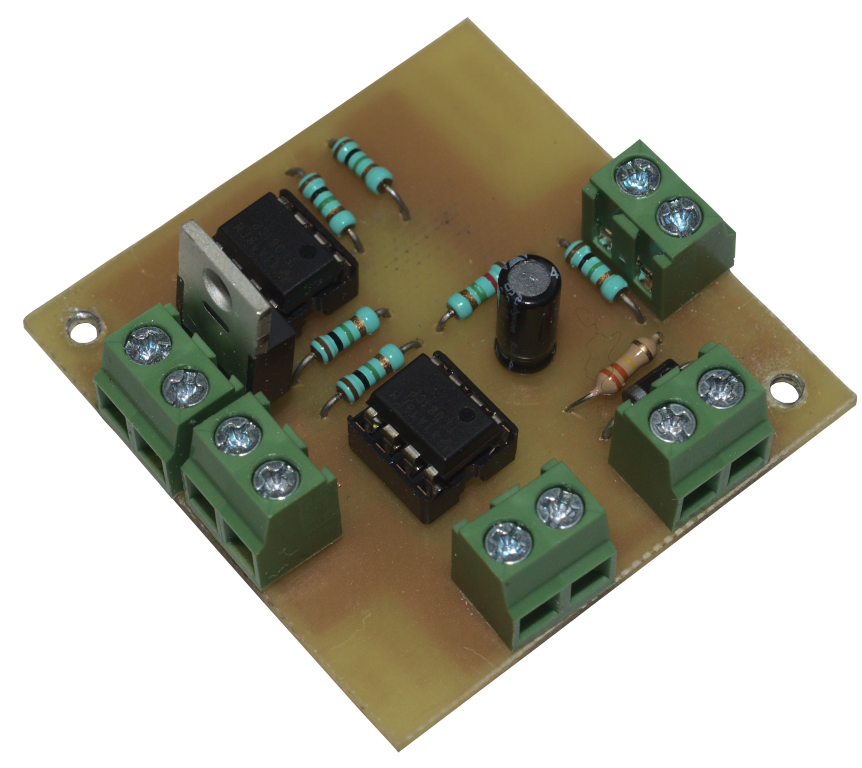
\includegraphics[width=0.9\textwidth]{Fotos/Platine_Relaischaltung.png}};
        \begin{scope}[x={(image.south east)},y={(image.north west)}]
            \draw[red,ultra thick,rounded corners,rotate around={30:(0.58,0.11)}] (0.58,0.11) rectangle (0.79,0.35);
            \draw[blue,ultra thick,rounded corners,rotate around={30:(0.77,0.28)}] (0.77,0.28) rectangle (0.97,0.51);
            \draw[orange,ultra thick,rounded corners,rotate around={37:(0.29,0.21)}] (0.29,0.21) rectangle (0.46,0.42);
            \draw[Green,ultra thick,rounded corners,rotate around={37:(0.16,0.38)}] (0.16,0.38) rectangle (0.34,0.55);
            \draw[violet,ultra thick,rounded corners,rotate around={40:(0.78,0.56)}] (0.78,0.56) rectangle (0.93,0.81);
        \end{scope}
    \end{tikzpicture}
    \captionof{figure}{Platine zur Relaisansteuerung}
\end{minipage}
\begin{minipage}{7.5cm}
    \textcolor{Green}{Hauptrelaisspule (A- \& GND) (J6)}\\
    \textcolor{blue}{Micro-Switches im Ladedeckel (J1)}\\
    \textcolor{orange}{Buck-Converter (nicht verwendet) (J2)}\\
    \textcolor{violet}{+30 V von geschalteter Relaisseite (J7)}\\
    \textcolor{red}{Konstante +30 V (J8)}\\
\end{minipage}\\

\textbf{Anmerkung:}\\
Die Relais der Buck-Converter werden nicht mehr, wie ursprünglich gedacht, über eine separate Zeitkonstante angesteuert, sondern verwenden nun den selben MOSFET wie das Hauptrelais. 

\newpage
\subsubsection{Funktionsweise}
Durch das Zusammenschalten der Akkus über den bereits zuvor gezeigten $10\,\mathrm{\Omega}$ Leistungswiderstand beginnen sich sowohl die Kondensatoren beider Motorregler und aller vier Buck-Converter sowie jener des sich auf der Platine befindlichen RC-Gliedes aufzuladen.\\
Erreicht dieser eine bestimmte Schwellspannung, wird das Hauptrelais mithilfe eines MOSFETs durch den Operationsverstärker der Komperatorschaltung aktiviert.\\
Dies führt zu einer Selbsthaltung des Relais, welche nur durch Betätigung des Not-Aus--Schalters oder das Öffnen einer der beiden Mikroschalter unterbrochen werden kann.\\
Der genaue Anschluss an die Leistungselektronik kann \autoref{fig:schaltLeistung} entnommen werden.
\subsubsection{Schaltplan}
\begin{figure}[h]
    \centering
    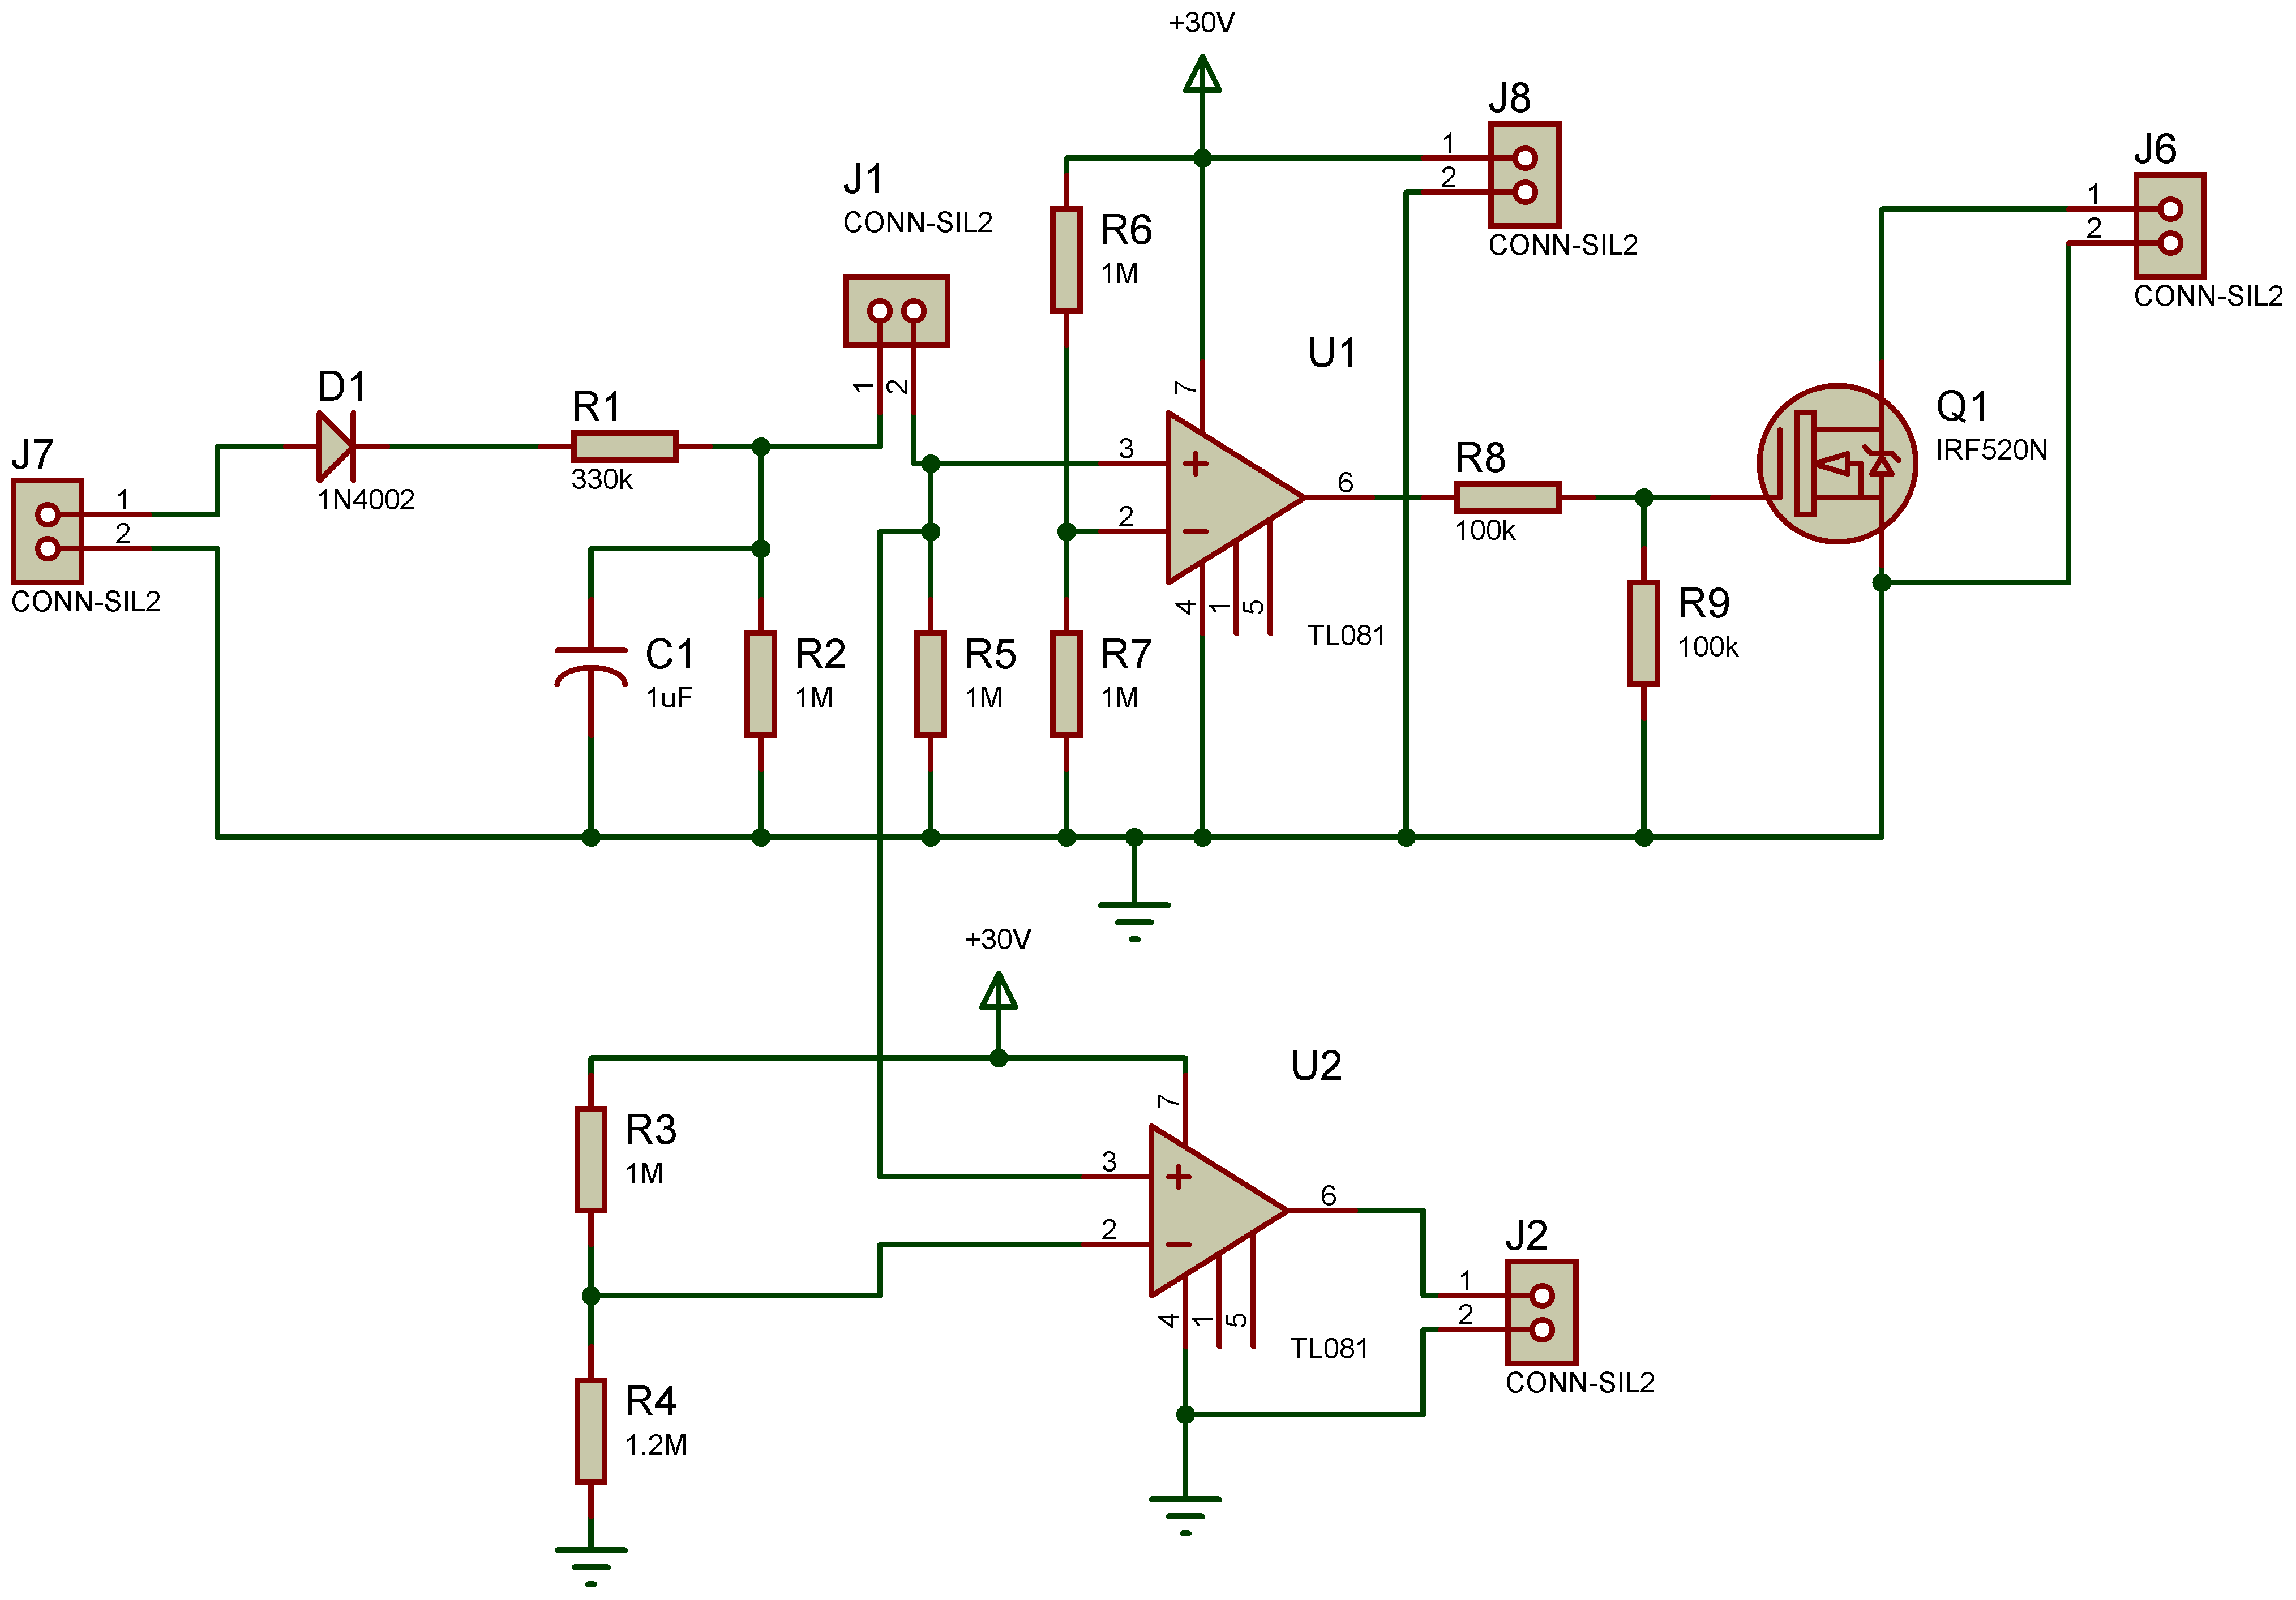
\includegraphics[width=0.99\textwidth]{../Proteus/Exports/Relaisansteuerung.png}
    \caption{Schaltplan der Platine zur Relaisansteuerung\label{fig:plat:relais}}
\end{figure}
\textbf{Anmerkung:}\\
Der OPV \textbf{U2} und die damit verbunde Klemme \textbf{J2} werden aufgrund einer nachträglichen Änderung im Schaltplan nicht mehr benötigt.
\newpage
\subsubsection{PCB-Layout}
\begin{figure}[h]
    \centering
    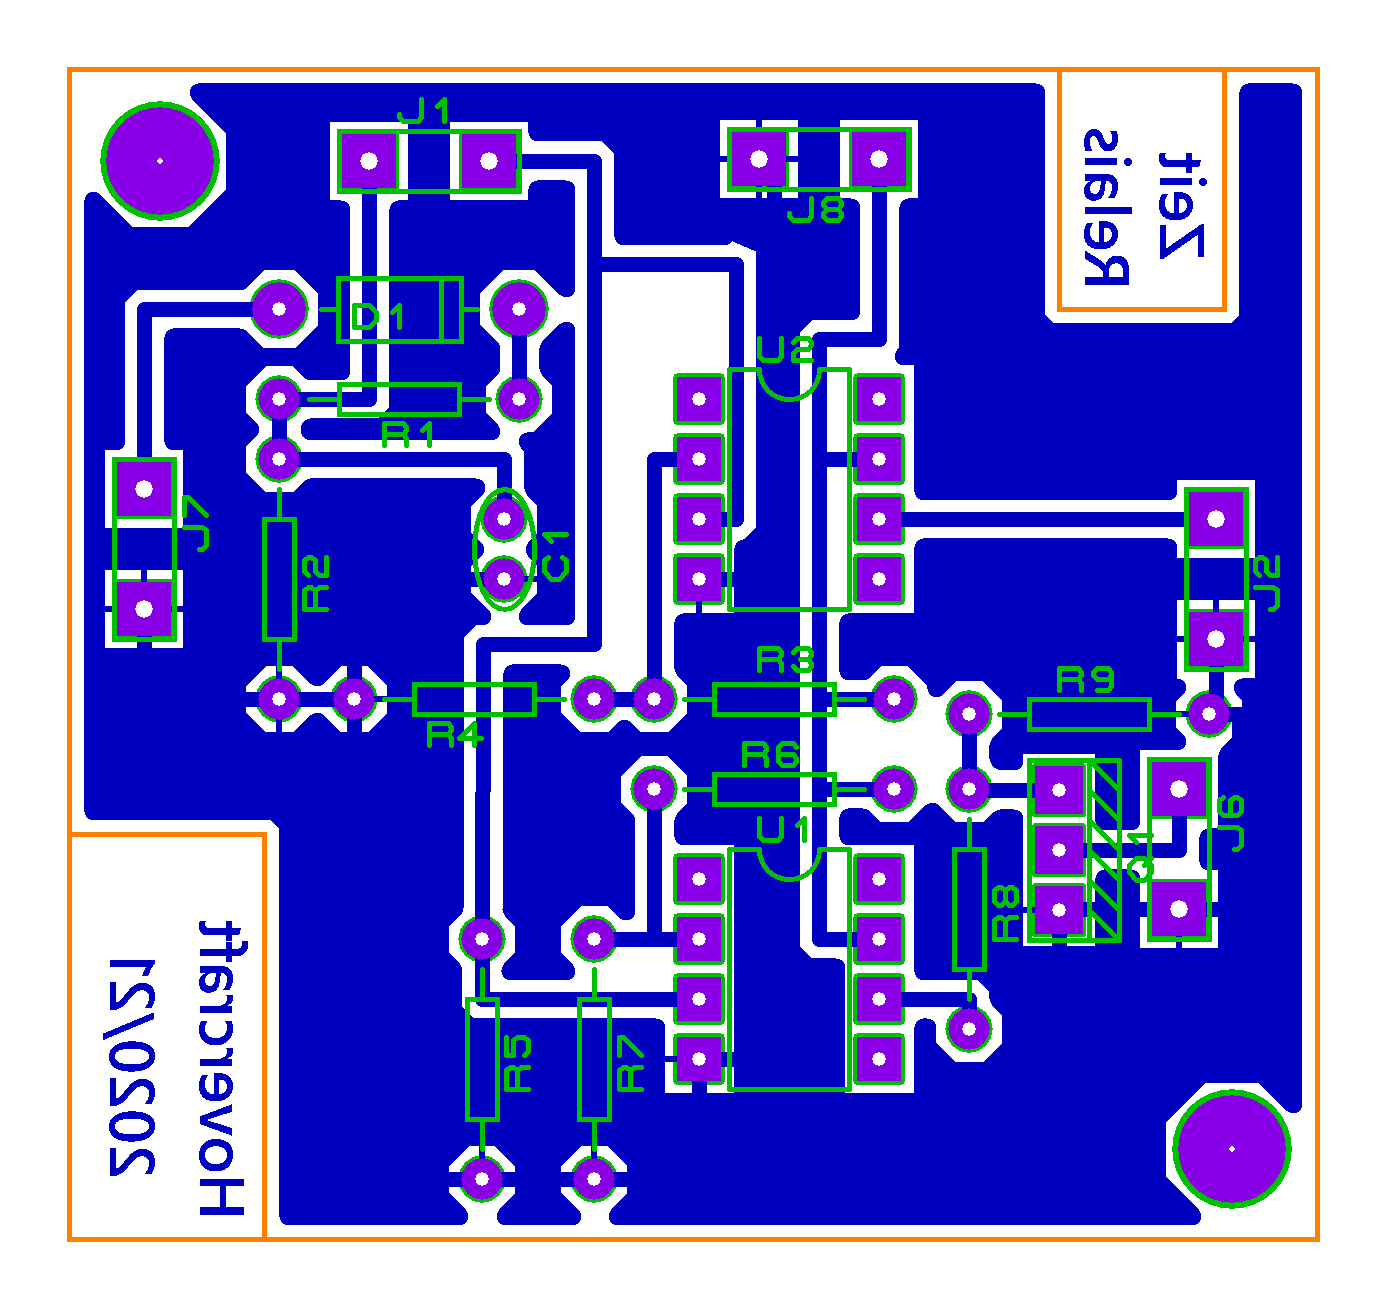
\includegraphics[width=0.95\textwidth]{../Proteus/Exports/Relaisansteuerung_PCB.png}
    \caption{PCB-Layout der Platine zur Relaisansteuerung}
\end{figure}
\newpage

\subsection{Platzierung am Boot}
Die Abbildungen \ref{fig:Platinen:Aufbau_Rechts} \& \ref{fig:Platinen:Aufbau_Links} zeigen die Positionen aller verbauten Platinen am Boot.\\

\begin{minipage}{\textwidth}
    \centering
    \begin{tikzpicture}
        \node[anchor=south west,inner sep=0] (image) at (0,0) {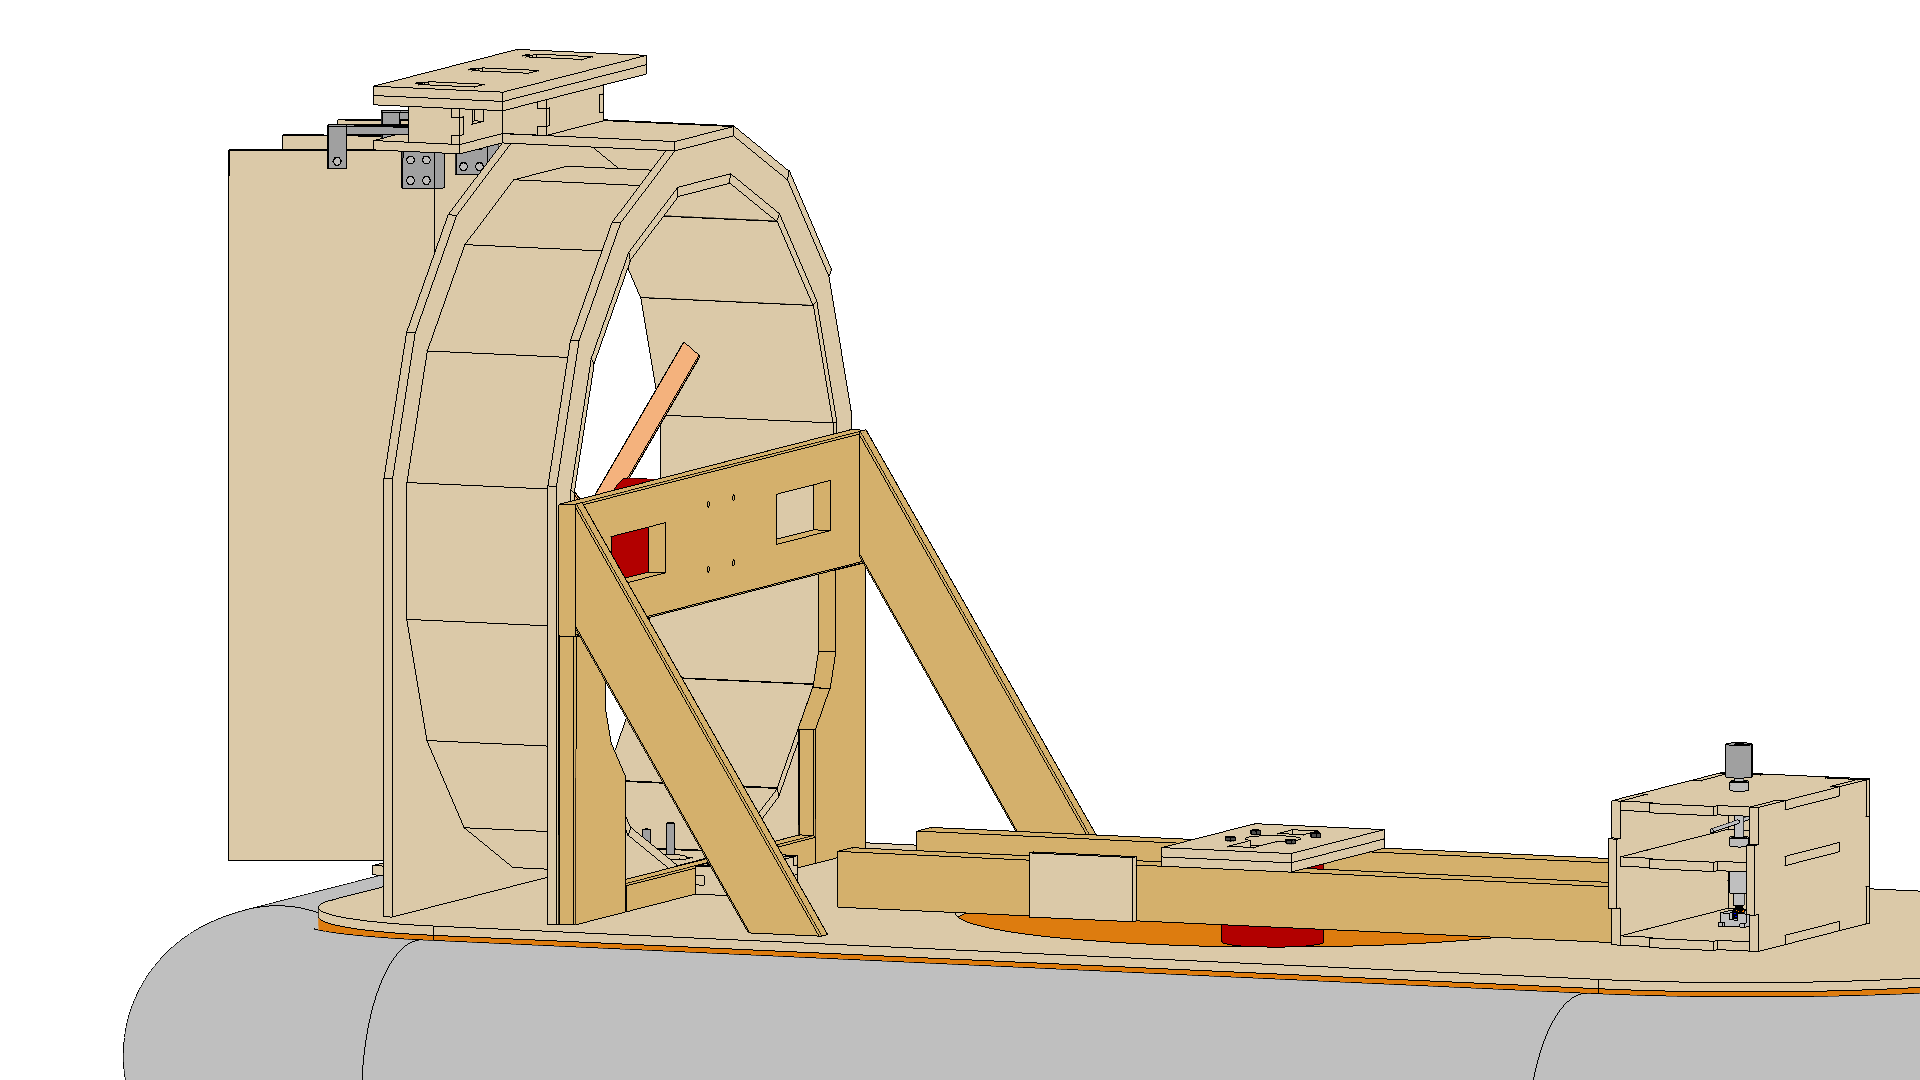
\includegraphics[width=0.85\textwidth]{../Inventor/PlatinenBilder/Seite1.png}};
        \begin{scope}[x={(image.south east)},y={(image.north west)}]
            \draw[blue,thick,->]  (0.66,0.85) -- (0.29,0.85) node [at start, above] {Temperatursensoren rechts} -- (0.22,0.40);
            \draw[black,thick,->]  (0.66,0.75) -- (0.29,0.75) node [at start, above] {Relaisansteuerung} -- (0.27,0.60);
            \draw[red,thick,->]  (0.66,0.65) -- (0.29,0.65) node [at start, above] {Regler-hinten Platine}  -- (0.27,0.51);
            \draw[black,thick,->]  (0.66,0.55) -- (0.5,0.55) node [at start, above] {Regler-unten Platine} -- (0.47,0.19);
            \draw[Green,thick,->]  (0.54,0.45) -- (0.78,0.45) node [midway, above] {Lenker Platine} -- (0.89,0.14);
        \end{scope}
    \end{tikzpicture}
    \captionof{figure}{Platinen auf der rechten Seite des Bootes}
    \label{fig:Platinen:Aufbau_Rechts}
\end{minipage}

\begin{minipage}{\textwidth}
    \centering
    \begin{tikzpicture}
        \node[anchor=south west,inner sep=0] (image) at (0,0) {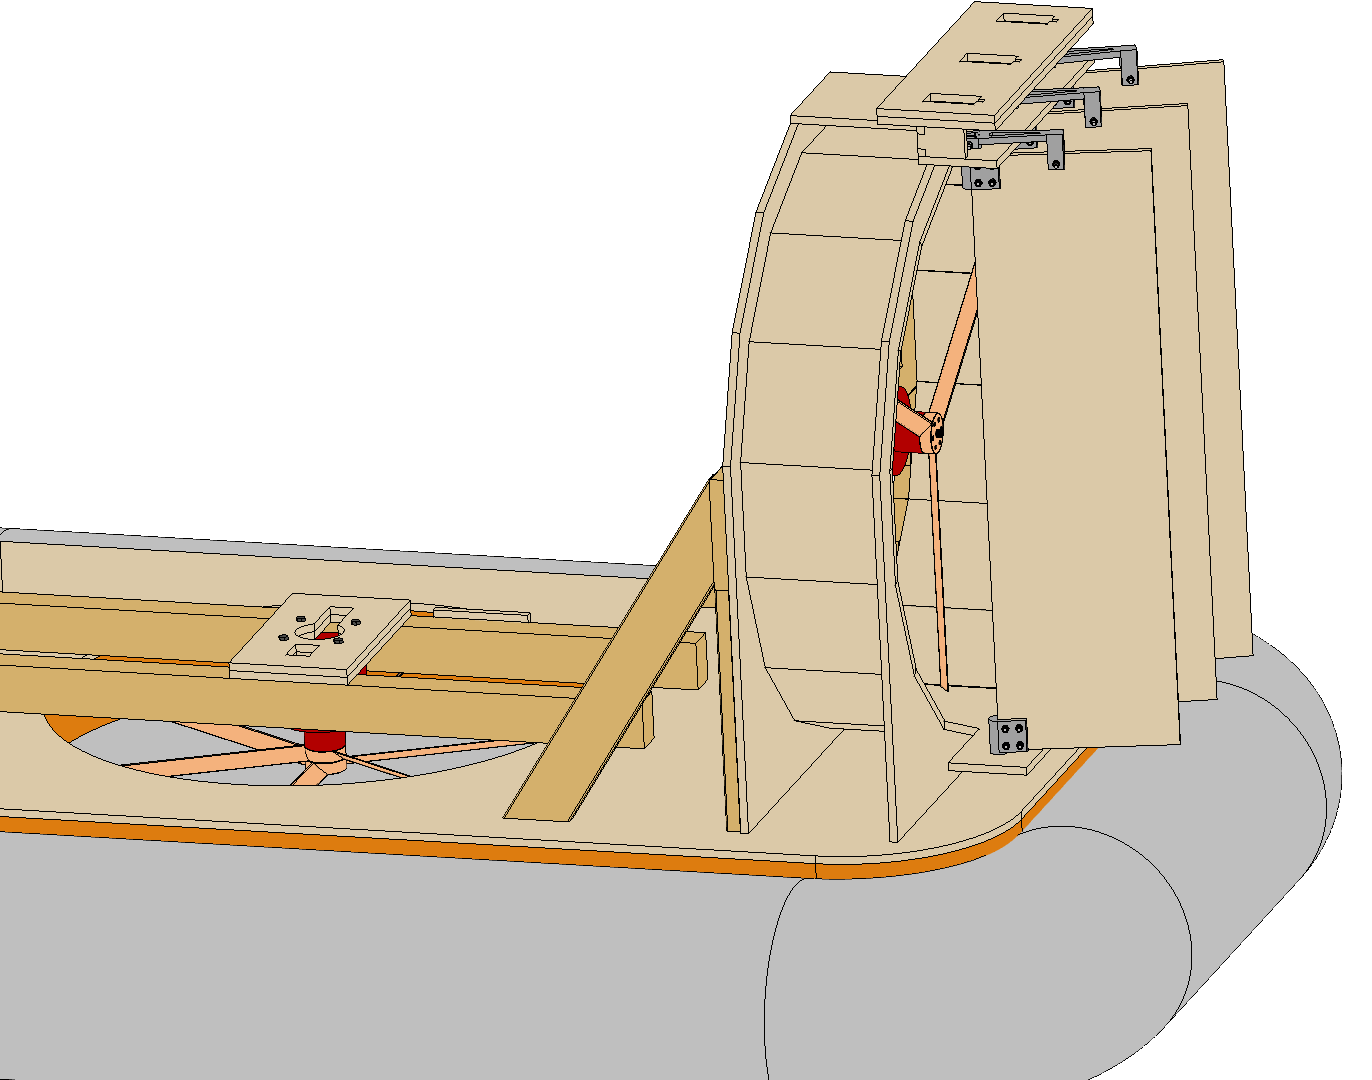
\includegraphics[width=0.85\textwidth]{../Inventor/PlatinenBilder/Seite2_2.png}};
        \begin{scope}[x={(image.south east)},y={(image.north west)}]
            \draw[red,thick,->]  (0.22,0.75) -- (0.5,0.75) node [midway, above] {Servo-ADC Platine}  -- (0.6,0.61);
            \draw[blue,thick,->]  (0.22,0.85) -- (0.5,0.85) node [midway, above] {Servo-Controller}  -- (0.61,0.81);
            \draw[black,thick,->]  (0.22,0.65) -- (0.49,0.65) node [near start, above] {Temperatursensoren links}  -- (0.545,0.42);
        \end{scope}
    \end{tikzpicture}
    \captionof{figure}{Platinen auf der linken Seite des Bootes}
    \label{fig:Platinen:Aufbau_Links}
\end{minipage}

\newpage
